\documentclass[a4paper,11pt]{article}
\usepackage{graphicx} % Required for inserting images
\usepackage{tikz}
\usepackage[french]{babel}
\usepackage[utf8]{inputenc}
\usepackage[T1]{fontenc}

\usepackage{hyperref}

\usepackage{listings}
\usepackage{graphicx}
\usepackage{hyperref}
\hypersetup{
    colorlinks=true,
    linkcolor=blue,
    filecolor=magenta,      
    urlcolor=cyan,
    pdftitle={Overleaf Example},
    pdfpagemode=FullScreen,
    }

\urlstyle{same}
\usepackage{fancyhdr}
\usetikzlibrary{positioning}
\usepackage{minted}
\usepackage{etoolbox}
\usepackage{xstring}
\usepackage{pgffor}
\usepackage{xstring}
\usepackage{wrapfig}
\usepackage{trimspaces}
\usepackage{cite}
\usepackage[a4paper,top=25mm]{geometry}
\usepackage[
    protrusion=true,
    activate={true,nocompatibility},
    final,
    tracking=true,
    kerning=true,
    spacing=true,
    factor=1100]{microtype}
\usepackage{setspace}

\renewcommand{\baselinestretch}{1} % Interligne simple
\setlength{\parskip}{1.0\baselineskip} % Espace entre paragraphes (1,5 lignes)

%% === Page Style ===
\pagestyle{fancy}
\usepackage[utf8]{inputenc}
\usepackage[french]{babel}
\usepackage{geometry}
\usepackage{listings}
\usepackage{color}
\usepackage{hyperref}
%% === NewCommand ==
\newcommand{\li}{\newline}
%% == Header/Footer ==
\fancyhf{}
\fancyhead[L]{\includegraphics[trim={0 200px 0 0},clip,height=30px]{unamur}}
\fancyhead[C]{\large{\textbf{Rétro-Ingénierie d'une base de donnée}}}
\fancyhead[R]{INFOM218\\\href{https://unamur.be}{\textcolor{black}{UNamur}}}
\fancyfoot[C]{\thepage}
\setlength{\headheight}{40pt}


\begin{document}


\begin{titlepage}

    \newcommand{\HRule}{\rule{\linewidth}{0.5mm}} % Defines a new command for the horizontal lines, change thickness here

    \center % Center everything on the page

    %----------------------------------------------------------------------------------------
    %	HEADING SECTIONS
    %----------------------------------------------------------------------------------------

    \textsc{\LARGE UNamur}\\[1.5cm] % Name of your university/college
    \includegraphics[scale=0.33]{unamur.jpg}\\[1cm] % Include a department/university logo - this will require the graphicx package
    \textsc{\Large Faculté d’informatique}\\[0.5cm] % Major heading such as course name
    \textsc{\large INFOM218:Evolution de systèmes logiciels}\\[0.5cm] % Minor heading such as course title

    %----------------------------------------------------------------------------------------
    %	TITLE SECTION
    %----------------------------------------------------------------------------------------

    \HRule \\[0.4cm]
    { \huge \bfseries Rétro-Ingénierie d'une base de donnée}\\[0.4cm] % Title of your document
    \HRule \\[1.5cm]

    %----------------------------------------------------------------------------------------
    %	AUTHOR SECTION
    %----------------------------------------------------------------------------------------

    \begin{minipage}{0.6\textwidth}
        \begin{flushleft} \large
            \emph{Auteurs:}\\
            Rosny  \textsc{Anderson Fodja Kouanga}\\
            Noé  \textsc{Pozza}\\
            Ryad  \textsc{HARITTANE}\\
            
        \end{flushleft}
       
        \begin{flushleft} \large
        \end{flushleft}

    \end{minipage}\\[2cm]

    % If you don't want a supervisor, uncomment the two lines below and remove the section above
    %\Large \emph{Author:}\\
    %John \textsc{Smith}\\[3cm] % Your name

    %----------------------------------------------------------------------------------------
    %	DATE SECTION
    %----------------------------------------------------------------------------------------

    {\large \today}\\[2cm] % Date, change the \today to a set date if you want to be precise

    \vfill % Fill the rest of the page with whitespace

\end{titlepage}

\newpage

\section*{Introduction}

Ce rapport documente l'analyse approfondie de la base de données de l'application Android open-source \textbf{Conversations}. En nous appuyant sur l'outil \textbf{SQLInspect}, nous avons étudié les interactions SQL présentes dans le code source pour reconstituer et analyser les schémas physiques et logiques de la base de données. Cette démarche vise à mieux comprendre la structure des données, leur utilisation dans l'application et les opportunités d'amélioration.

Le code source de \textbf{Conversations}, ainsi que les résultats détaillés de notre analyse, sont centralisés dans un dépôt GitHub dédié : 
\texttt{\href{https://github.com/NPozzaUNamur/Evolution_Group4}{lien vers le repo}}. Il constitue une ressource complète pour reproduire nos étapes, explorer le projet ou y contribuer.

Le rapport est structuré comme suit :
Dans un premier temps, nous procédons à l'analyse du code DDL pour identifier et reconstruire les structures de la base de données de l'application. Ensuite, nous présentons le schéma physique obtenu, tout en explorant les relations implicites et explicites entre les différentes entités. Une section est dédiée aux propositions d'améliorations, incluant la découverte de clés étrangères implicites et l'ajout de contraintes pour renforcer l'intégrité des données. Nous examinons ensuite l'impact des scénarios d'évolution sur la structure de la base de données et sur le code source de l'application. Enfin, nous concluons en évaluant la qualité globale de la base de données et en formulant des recommandations pour sa maintenance et son évolution futures.

En suivant cette approche méthodique, nous visons à fournir une compréhension approfondie de la base de données utilisée dans \textbf{Conversations} et à proposer des solutions concrètes pour la rendre plus robuste, efficace et évolutive.


\section*{Analyse du code DDL}

Dans cette section, nous allons commencer notre rétro-ingénierie de base de donnée par l'analyse du code DDL présent dans la code base de l'application. Ceci nous permettra de ressortir des informations tant bien sur l'aspect technique que sur la signification des données. Pour faciliter notre travail, on a aggloméré les informations dans un fichier \textit{MarkDown} nommé \textit{analyse.md},disponible sur notre répertoire. 

\subsection*{Classe d'intérêt}

En premier lieu, il est nécessaire de trouver la, ou les, parties de l'application responsable de la gestion de la base de données.
Le rapport fourni par SQLInspect nous dirige vers deux classes: \textit{DatabaseBackend} et \textit{UnifiedPushDatabase}.
Le point commun de ces deux classes est qu'elles sont  filles de la classe abstraite \href{https://developer.android.com/reference/android/database/sqlite/SQLiteOpenHelper}{\textit{SQLiteOpenHelper}}. Cette classe permet la gestion de bases de données SQL.

Sachant que le moteur de base de données utilisé est SQLite, ce qui est courant pour une application mobile, nous constatons qu'il existe deux bases de données distinctes. Cette conclusion découle de l'existence de deux classes distinctes implémentant la classe \textit{SQLiteOpenHelper}, chacune étant responsable de la gestion d'une base de données spécifique.

\subsection*{\textit{DatabaseBackend}}

La classe \textit{DatabaseBackend} définit la base de données nommée \textit{History}. Celle-ci semble avoir la responsabilité de contenir les données relatives aux messages, à la sécurité, aux contacts et aux serveurs. Elle est donc la base de données principale de cette application Android.\\
Elle contient 11 tables différentes. Nous avons reconstitué les requêtes DDL à l'origine des classes afin de pouvoir recréer le schéma physique. Voici la liste:

    %*************** 
\subsubsection*{Contact}
Contient les informations sur un contact. Elle fait partie de la fonctionnalité de gestion des contacts. Il y est définie une relation avec la table \textit{Account}. L'application permettant de gérer plusieurs comptes, il est nécessaire de lier un contact à un compte.

Un contact peut être aussi un groupe, ou plus formellement, un \href{https://xmpp.org/extensions/xep-0045.html}{\textit{Multi-User Chat (MUC)}}. C'est une fonctionnalité du protocole XMPP, qui permet de créer des salons de discussion.

D'après nos analyses , cette table ne possède pas de clé primaire explicite, mais des contraintes d'unicité sont appliquées sur les colonnes \textit{accountUuid} et \textit{jid}. Cela vise à empêcher l'enregistrement de doublons pour un même contact. Cependant, il apparaît que ces colonnes, \textit{jid} et \textit{accountUuid}, sont utilisées implicitement comme une clé primaire\footnote{eu.siacs.conversations.entities.Contact 115: \textit{Jid.of} n'accepte pas de valeur null}. Cela peut poser un problème, car la valeur \textit{null} est permise pour ces colonnes, ce qui pourrait nuire à l'intégrité des données.

Le champ \textit{jid} (mis pour \textit{Jabber ID}) est un identifiant unique utilisé dans le protocole XMPP, un protocole de messagerie instantanée sur lequel repose l'application.

De plus, il est intéressant de noter que cette table est l'une des rares à ne pas hériter de la classe \textit{AbstractEntity}, ce qui se traduit par l'absence de la colonne \textit{uuid}, habituellement utilisée comme identifiant unique dans les autres entités.

\textbf{DDL}
\begin{lstlisting}
create table contacts(
    accountUuid TEXT,
    servername TEXT, 
    systemname TEXT,
    presence_name TEXT,
    jid TEXT,
    pgpkey TEXT,
    photouri TEXT,
    options NUMBER,
    systemaccount NUMBER,
    avatar TEXT,
    last_presence TEXT,
    last_time NUMBER, 
    rtpCapability TEXT,
    groups TEXT, 
    
    FOREIGN KEY(accountUuid) REFERENCES accounts(uuid) 
     ON DELETE CASCADE,
    UNIQUE(accountUuid, jid) ON CONFLICT REPLACE
);
\end{lstlisting}
%***************
\subsubsection*{Account}
Contient les informations sur un compte. Table centrale de cette base de données, elle permet la gestion des comptes XMPP. Il est donc à noter que les colonnes \textit{username}, \textit{server} et \textit{ressource} font donc référence au \textit{jid} utilisé par le protocole XMPP. Il prend la forme de \textit{username@server/ressource}\footnote{\href{https://xmpp.org/extensions/xep-0029.html}{xmpp documentation}}.

Tout comme pour la table \textit{Contact}, la colonne \textit{jid} semble ne pas pouvoir être \textit{null}. Une requête exécutée avec une valeur \textit{null} pour les colonnes \textit{username} ou \textit{server} entraîne une erreur\footnote{eu.siacs.conversations.entities.Account 176-180: \textit{Jid.of} n'accepte pas de valeur \textit{null}}. Cela confirme implicitement que \textit{jid} doit être bien formé et non \textit{null} pour garantir le fonctionnement correct de l'application.

Cette table possède cependant une clé primaire explicite, \textit{uuid}, qui est une chaîne de caractères générée aléatoirement.

\textbf{DDL}
\begin{lstlisting}
create table accounts(
    uuid TEXT PRIMARY KEY,
    username TEXT,
    server TEXT,
    password TEXT,
    display_name TEXT,
    status TEXT,
    status_message TEXT,
    rosterversion TEXT,
    options NUMBER,
    avatar TEXT,
    keys TEXT,
    hostname TEXT,
    resource TEXT,
    pinned_mechanism TEXT,
    pinned_channel_binding TEXT,
    fast_mechanism TEXT,
    fast_token TEXT,
    port NUMBER DEFAULT 5222
);
\end{lstlisting}
%***************
\subsubsection*{Conversation}

Cette table contient les informations sur une conversation entre un compte et un contact. Elle est donc une table de liaison entre les tables \textit{Account} et \textit{Contact}. Elle contient aussi des informations sur le nom de la conversation, le statut, le mode et des attributs.

Deux colonnes se reportent implicitement à la table \textit{Contact}. Il s'agit de \textit{contactUuid} et \textit{contactJid}. La première colonne est étrange , compte  tenu du fait que la table \textit{Contact} ne contient pas de colonne \textit{uuid}. Il est possible que cette colonne soit une erreur de conception. La seconde colonne, \textit{contactJid}, est une référence au \textit{jid} du contact (qui peut donc être un groupe). Ce qui tend à confirmer que le \textit{jid} est une clé primaire implicite de la table \textit{Contact}\footnote{eu.siacs.conversations.entities.Conversation 673: Seule la colonne \textit{contactJid} est utilisé comme lien avec la table \textit{Contact}}.

Fille de la classe \textit{AbstractEntity}, elle contient une clé primaire , \textit{uuid}, qui est une chaîne de caractères générée aléatoirement.

\textbf{DDL}
\begin{lstlisting}
create table conversations (
    uuid TEXT PRIMARY KEY,
    name TEXT,
    contactUuid TEXT,
    accountUuid TEXT,
    contactJid TEXT,
    created NUMBER,
    status NUMBER,
    mode NUMBER,
    attributes TEXT, 
    
    FOREIGN KEY(accountUuid) REFERENCES accounts(uuid)
     ON DELETE CASCADE
);
\end{lstlisting}
%***************
\subsubsection*{Message}

Contient les informations sur un message. Il est à noter que la colonne \textit{conversationUuid} est une clé étrangère vers la table \textit{Conversation}. Cette table contient aussi des informations sur le contenu du message et sur l'aspect technique du message, comme le type, le statut, le temps d'envoi, etc.

La colonne \textit{trueCounterpart} est une colonne qui sert à stocker le \textit{jid} du contact, lorsque la conversation est un groupe. Cela permet de savoir qui a envoyé le message. Elle est donc en un sens une clé étrangère implicite vers la table \textit{Contact}\footnote{eu.siacs.conversations.entities.Message 352: \textit{trueCounterpart} est utilisé pour la relation avec \textit{Contact}}.

Une table virtuelle est aussi présente. Sous le nom de \textit{messages\_index}, elle permet une recherche rapide des messages. Elle est donc une table de cache. Afin de maintenir à jour cette table, des triggers sont utilisés afin que chaque modification, ajout, suppression de la table \textit{Message} soit répercutée sur la table \textit{messages\_index}.

\textbf{DDL}
\begin{lstlisting}
create table messages(
    uuid TEXT PRIMARY KEY,
    conversationUuid TEXT,
    timeSent NUMBER,
    counterpart TEXT,
    trueCounterpart TEXT,
    body TEXT,
    encryption NUMBER,
    status NUMBER,
    type NUMBER,
    relativeFilePath TEXT,
    serverMsgId TEXT,
    axolotl_fingerprint TEXT,
    carbon INTEGER,
    edited TEXT,
    read NUMBER DEFAULT 1,
    oob INTEGER,
    errorMsg TEXT,
    readByMarkers TEXT,
    markable NUMBER DEFAULT 0,
    deleted NUMBER DEFAULT 0,
    bodyLanguage TEXT,
    occupantId TEXT,
    reactions TEXT,
    remoteMsgId TEXT, 
    
    FOREIGN KEY(conversationUuid) REFERENCES conversations(uuid) 
     ON DELETE CASCADE
);
\end{lstlisting}
%***************
\subsubsection*{Identity}

Table servant à stocker les informations sur les identités. Il s'agit des informations sur les clés cryptographiques. Elle contient des informations sur le compte, le nom, la clé, le certificat, la confiance, etc.

Étant liée à l'aspect sécurité de l'application, nous n'allons pas nous attarder sur les détails de cette table.

\textbf{DDL}
\begin{lstlisting}
CREATE TABLE identities(
    account TEXT,
    name TEXT,
    ownkey INTEGER,
    fingerprint TEXT,
    certificate BLOB,
    trust TEXT,
    active NUMBER,
    last_activation NUMBER,
    key TEXT,
    
    FOREIGN KEY(account) REFERENCES accounts(uuid)
     ON DELETE CASCADE
    UNIQUE( account, name, fingerprint)
     ON CONFLICT IGNORE
);
\end{lstlisting}
%***************
\subsubsection*{Session}

Table servant à stocker les informations sur les sessions. Elle contient des informations sur le compte, le nom, l'identifiant du device, la clé, etc.

Étant liée à l'aspect sécurité de l'application, nous n'allons pas nous attarder sur les détails de cette table.

\textbf{DDL}
\begin{lstlisting}
CREATE TABLE sessions(
    account TEXT,
    name TEXT,
    device_id INTEGER,
    key TEXT,
    
    FOREIGN KEY(account) REFERENCES accounts(uuid)
     ON DELETE CASCADE,
    UNIQUE( account, name, device_id)
     ON CONFLICT REPLACE
);
\end{lstlisting}
%***************
\subsubsection*{Prekey}

Étant liée à l'aspect sécurité de l'application, nous n'allons pas nous attarder sur les détails de cette table.

\textbf{DDL}
\begin{lstlisting}
CREATE TABLE prekeys(
    account TEXT,
    id INTEGER,
    key TEXT,
    FOREIGN KEY(account) REFERENCES accounts(uuid)
     ON DELETE CASCADE,
    UNIQUE( account, id)
     ON CONFLICT REPLACE
);
\end{lstlisting}
%***************
\subsubsection*{Signed Prekey}

Étant liée à l'aspect sécurité de l'application, nous n'allons pas nous attarder sur les détails de cette table.

\textbf{DDL}
\begin{lstlisting}
CREATE TABLE signed_prekeys(
    account TEXT,
    id INTEGER,
    key TEXT,
    
    FOREIGN KEY(account) REFERENCES accounts(uuid)
     ON DELETE CASCADE,
    UNIQUE( account, id)
     ON CONFLICT REPLACE
);
\end{lstlisting}
%***************
\subsubsection*{Resolver Result}

Cette table contient les résultats de la résolution DNS. Elle contient des informations sur le domaine, le nom d'hôte, l'adresse IP, la priorité, le TLS direct, l'authentification, le port, etc.

Elle permet à l'application de garder en mémoire les résultats de résolution DNS pour une utilisation ultérieure.

\textbf{DDL}
\begin{lstlisting}
create table resolver_results(
    domain TEXT,
    hostname TEXT,
    ip BLOB,
    priority NUMBER,
    directTls NUMBER,
    authenticated NUMBER,
    port NUMBER,
    
    UNIQUE(domain) ON CONFLICT REPLACE
);
\end{lstlisting}
%***************
\subsubsection*{Discovery Result}

Cette table contient le résultat des découvertes de services disponibles . Elle est liée aux fonctionnalités de XMPP\footnote{\href{https://xmpp.org/extensions/xep-0030.html}{XMPP Documentation}}.

\textbf{DDL}
\begin{lstlisting}
create table discovery_results(
    hash TEXT,
    ver TEXT,
    result TEXT,
    
    UNIQUE(hash, ver) ON CONFLICT REPLACE
);
\end{lstlisting}
%***************
\subsubsection*{Presence Template}

Contient les informations sur les patterns de présence. C'est-à-dire, un message que l'utilisateur veut afficher, et un statut. Ce statut peut être \textit{chat}, \textit{online}, \textit{away}, \textit{offline}, etc\footnote{eu.siacs.conversations.entities.Presence 12}.

On constate qu'aucune des colonnes n'est une clé primaire. Cependant, une contrainte d'unicité est appliquée sur les colonnes \textit{message} et \textit{status}. Cela permet de ne pas avoir deux fois le même message avec le même statut.

\textbf{DDL}
\begin{lstlisting}
CREATE TABLE presence_templates(
    uuid TEXT,
    last_used NUMBER,
    message TEXT,
    status TEXT,
    
    UNIQUE(message,status) ON CONFLICT REPLACE
);
\end{lstlisting}
%***************

\subsection*{\textit{UnifiedPushDatabase}}

Cette classe définit la base de données nommée \textit{unified-push-distributor}. Celle-ci semble avoir la responsabilité de contenir les données relatives aux notifications push. Elle ne contient qu'une seule table, \textit{push}, qui contient les informations sur les notifications push.

\subsubsection*{Push}

Contient les informations sur une notification push. Elle est reliée au système de notification d'Android .

Elle semble liée à la table \textit{Account}, mais il n'y a pas de clé étrangère déclarée. Cependant, la colonne \textit{account} est utilisée pour se référer à \textit{accounts.uuid}, suggérant une clé étrangère implicite. L'utilisation de \textit{account} comme clé étrangère implicite est sans doute contrainte par le fait que cette table et la table \textit{Account} sont dans des bases de données différentes.

\textbf{DDL}
\begin{lstlisting}
CREATE TABLE push (
	account TEXT,
	transport TEXT,
	application TEXT NOT NULL,
	instance TEXT NOT NULL UNIQUE,
	endpoint TEXT,
	expiration NUMBER DEFAULT 0
);
\end{lstlisting}

\section*{Analyse du Schéma et des Requêtes}
Cette section détaille  l'analyse des requêtes utilisées dans l'application. Elle met en évidence la découverte de clés étrangères implicites non représentées explicitement dans le schéma physique obtenu. Nous examinons également dans quelle mesure les clés étrangères explicites peuvent être inférées à partir du schéma physique ou des requêtes utilisées dans l'application. De plus, cette section explore la possibilité de découvrir des clés étrangères implicites qui ne sont pas explicitement déclarées. L'objectif est de compléter le schéma logique en identifiant et en ajoutant ces relations non documentées, afin de renforcer l'intégrité référentielle et la clarté du modèle de données.

\subsection*{Résultats}
\subsubsection*{Inférence des Clés Étrangères Explicites}
Pour ce faire, nous proposons de procéder en deux étapes : tout d'abord, en examinant le schéma physique (en se basant sur les noms et types des colonnes) pour identifier d'éventuelles clés étrangères. Ensuite, en analysant les requêtes SQL, notamment les jointures, les relations entre sorties et entrées des requêtes, afin de confirmer ou de  découvrir des liens implicites supplémentaires entre les tables.

En analysant le schéma physique, on observe qu'une grande majorité des tables contiennent une colonne \texttt{account} de type \texttt{TEXT}. Par déduction logique, et en nous appuyant sur les résultats fournis par SQLInspect ainsi que sur les jointures détectées, nous pouvons supposer que ces colonnes \texttt{account} font référence à la colonne \texttt{Account.uuid}. Cette relation semble être une clé étrangère implicite, bien qu'elle ne soit pas explicitement définie dans le schéma physique. 

De plus, plusieurs relations implicites entre les tables peuvent être identifiées :

La table \texttt{Account} contient une colonne \textbf{hostname}, que l'on peut relier logiquement à la colonne \textbf{hostname} de la table \texttt{Resolver\_Results}. Cette liaison pourrait permettre de retrouver les résultats de résolutions DNS associés à un compte donné.

La table \texttt{Conversations} possède une colonne \textbf{ContactJid}, qui semble être liée à la colonne \textbf{ContactJid} de la table \texttt{Contacts}. Cette relation établit une correspondance entre une conversation et le contact auquel elle est associée.

La table \texttt{Message} comprend une colonne \textbf{ConversationUuid}, que l'on relie à la colonne \textbf{uuid} de la table \texttt{Conversations}. Cette relation lie chaque message à une conversation spécifique, garantissant ainsi la cohérence des données entre ces deux entités.

En ce qui concerne les requêtes, elles ne fournissent aucune information supplémentaire, ni sur les jointures ni sur d'autres relations. Sans une analyse plus approfondie du programme, il n'est pas possible d'en tirer des conclusions supplémentaires.

Calculons maintenant le recall et la précision comme cela est fait dans le cours. Pour ce qui est de la précision c'est simple, c'est \textbf{100\%}, en effet toutes les clés étrangères sont des vraies et aucune n'est un faux positif. 

Par contre pour le recall étant donné que l'on n'a pas trouvé toutes les clés, il faut faire les calculs par rapport aux nombres de clés totales.
On a déduits du schéma \textbf{10 clés étrangères} pour un total de \textbf{14 clés étrangères}. Notre recall est donc évalué à \textbf{71,42\%}.

\subsubsection*{Découverte de Clés Étrangères Implicites Additionnelles}
Nous avons analysé les requêtes SQL pour identifier des utilisations de colonnes qui fonctionnent comme des clés étrangères mais qui ne sont pas formellement définies comme telles dans les déclarations de table.

\begin{itemize}
    \item \textbf{Relation \texttt{push → accounts}:}
    \begin{itemize}
        \item \textbf{Requête:} \texttt{SELECT EXISTS(SELECT endpoint FROM push WHERE account = ...)}
        \item \textbf{Construction:} \texttt{push.account} → \texttt{accounts.uuid}
        \item \textbf{Justification:} Cette requête utilise \texttt{push.account} pour se référer à \texttt{accounts.uuid}, suggérant une clé étrangère entre ces deux tables. 
    \end{itemize}
    \item \textbf{Relation \texttt{conversations.contactJid → contacts.jid}:}
    \begin{itemize}
        \item \textbf{Requête:} Utilisation de \texttt{contactJid} dans la classe \texttt{Conversation.java} (ligne 673).
        \item \textbf{Construction:} \texttt{conversations.contactJid} → \texttt{contacts.jid}
        \item \textbf{Justification:} \texttt{contactJid} est utilisé comme lien avec \texttt{contacts.jid} dans la logique de l'application. Seule la colonne \texttt{contactJid} est utilisée pour établir cette relation, tandis que \texttt{contactUuid} reste inutilisée, ce qui souligne une dépendance implicite.
    \end{itemize}
    \item \textbf{Relation \texttt{messages → contacts}:}
    \begin{itemize}
        \item \textbf{Requête:} Références dans \texttt{Message.java} (lignes 344-355).
        \item \textbf{Construction:} \texttt{messages.trueCounterpart} → \texttt{contacts.jid}
        \item \textbf{Justification:} \texttt{trueCounterpart} est utilisé pour référencer \texttt{contacts.jid}, dépendant du mode de conversation (un-à-un ou groupe). Si la conversation est entre deux personnes, \texttt{trueCounterpart} fait directement référence à \texttt{null}. Sinon, dans un contexte de groupe, \texttt{trueCounterpart} recherche l'identité appropriée dans la liste des contacts.
    \end{itemize}
    \item \textbf{Relation \texttt{messages → contacts}:}
    \begin{itemize}
    \item \textbf{Construction:} \texttt{messages.counterpart} → \texttt{contacts.jid}
    \item \textbf{Justification:} \texttt{counterpart} est utilisé pour définir le destinataire principal d'un message en fonction du type de conversation défini dans \texttt{Conversations.mode} (individuelle, privée ou de groupe). 
    \begin{itemize}
        \item Dans une conversation individuelle (\texttt{Conversation.MODE\_SINGLE}), \texttt{counterpart} fait directement référence au \texttt{jid} du contact avec lequel l'utilisateur échange. Ce JID est utilisé pour définir la destination du paquet XMPP via la méthode \texttt{packet.setTo()}.
        \item Dans une conversation privée au sein d'un groupe (\texttt{message.isPrivateMessage()}), \texttt{counterpart} fait référence au JID complet (\texttt{FullJid}) du membre du groupe recevant le message privé.
        \item Dans une conversation de groupe standard (\texttt{Type.GROUPCHAT}), \texttt{counterpart} correspond au \texttt{jid} du groupe (\texttt{asBareJid()}), ce qui définit l'ensemble du groupe comme destinataire du message.
    \end{itemize}
        \end{itemize}
    \item \textbf{Relation \texttt{sessions → contacts ou Account}:}
    \begin{itemize}
        \item \textbf{Requête:} Références dans \texttt{AxolotlService.java}.
        \item \textbf{Construction:} \texttt{sessions.name} → \texttt{contacts.jid} ou \texttt{accounts.jid}
        \item \textbf{Justification:} \texttt{name} dans la table \texttt{sessions} est utilisé pour identifier l'origine d'une session OMEMO, en fonction du type de JID (contact ou compte local).
        \begin{itemize}
            \item Lorsque la session concerne un contact, \texttt{name} est initialisé à partir de \texttt{contact.getJid()} via la méthode \texttt{findSessionsForContact()}. Cela correspond au JID complet du contact.
            \item Lorsque la session concerne l'utilisateur local, \texttt{name} est défini via 
            \texttt{account.getJid().asBareJid()
            .toString()} dans \texttt{getOwnAxolotlAddress()}. Cela correspond au JID sans ressource (bare JID) de l'utilisateur. et des méthodes comme \texttt{buildSessionFromPEP(final SignalProtocolAddress address, OnSessionBuildFromPep callback)} montre qu'une session peut s'ouvrir avec son propre compte sur un autre device (différents \texttt{device\_id}).
            \item Cette dualité permet de stocker dans une même structure (la table \texttt{sessions}) des sessions pour les contacts ainsi que les sessions propres à l'utilisateur local, tout en distinguant ces deux cas selon le contexte.
        \end{itemize}
    \end{itemize}
        \item \textbf{Relation \texttt{identities → accounts et contacts}:}
\begin{itemize}
    \item \textbf{Construction:} \texttt{identities.name} → \texttt{accountsjid (= Account.name@Account.server)} et \texttt{contacts.jid}, \texttt{identities.account} → \texttt{accounts.uuid}.
    \item \textbf{Justification:} 
    \begin{itemize}
        \item Dans le cas d’un \texttt{Account JID}, la requête utilise \texttt{name} pour rechercher les clés associées à l'utilisateur local via son \texttt{accounts.jid} (exemple : \texttt{loadOwnIdentityKeyPair} dans \texttt{DatabaseBackend.java}). De plus, \texttt{identities.account} relie cette identité à un compte spécifique via \texttt{accounts.uuid}.
        \item Dans le cas d’un \texttt{Contact JID}, \texttt{name} fait référence à \texttt{contacts.jid}, comme illustré dans la méthode \texttt{loadIdentityKeys}, qui récupère les clés d’un contact donné.
        \item Cette dualité démontre que la table \texttt{identities} est liée à la fois à \texttt{accounts} et \texttt{contacts} en fonction du contexte d’utilisation.
    \end{itemize}
\end{itemize}

    \end{itemize}




    % add conversation.contactJid -> contact : id de contact qui est implicite qui est pas clairement definie dans le schema on peut faire de lien avec conversation dans le fichier eu.siacs.conversations.entities.Conversation 673 : Seule la colonne contactJid est utilisé comme lien avec la table Contact contactuuuid ne sert pratiquement pas 
    % add message.trueCounterpart -> contact : eu.siacs.conversations.entities.message.java 344 si la conversation est une personne a une autre on recupere le contact si non donc c'est un groupe on recupere le recherche le contact dans la liste de contact 


La présence de clés étrangères non déclarées, comme celle entre \texttt{push} et \texttt{accounts}, indique que le schéma physique pourrait être amélioré pour expliciter ces relations, ce qui renforcerait la compréhension et la gestion de la base de données. L'ajout de cette clé au schéma logique aidera à maintenir l'intégrité référentielle et à optimiser les performances des requêtes.

\subsection*{Brève description du Schéma Physique (PS)}

Dans cette section, il s'agira de donner une brève description du schéma physique se trouvant sur notre repository Git dans le fichier /analyse/schema/schema\_physique.drawio. Les autres schémas se trouvant aussi  sur notre repository .

La principale différence observable par rapport à un schéma classique réside dans la représentation des liaisons de clés étrangères. Dans ce cas, les clés étrangères implicites sont représentées par des traits en pointillés noirs, tandis que les traits en pointillés bleus indiquent des clés étrangères implicites référencées sur deux colonnes d'une même table. Par exemple, la colonne \texttt{Identities.name} référence simultanément \texttt{Account.username} et \texttt{Account.server}.

La table \texttt{message\_index} est une table virtuelle conçue pour faciliter les recherches rapides de messages. Elle agit comme un index spécialisé, optimisant les performances lors de requêtes complexes ou fréquentes sur les messages.

Il y a deux bases de données, l'une contenant toute l'information \texttt{History} et l'autre servant pour les notifications seulement \texttt{Unified-Push-Distributor}.

\begin{center}
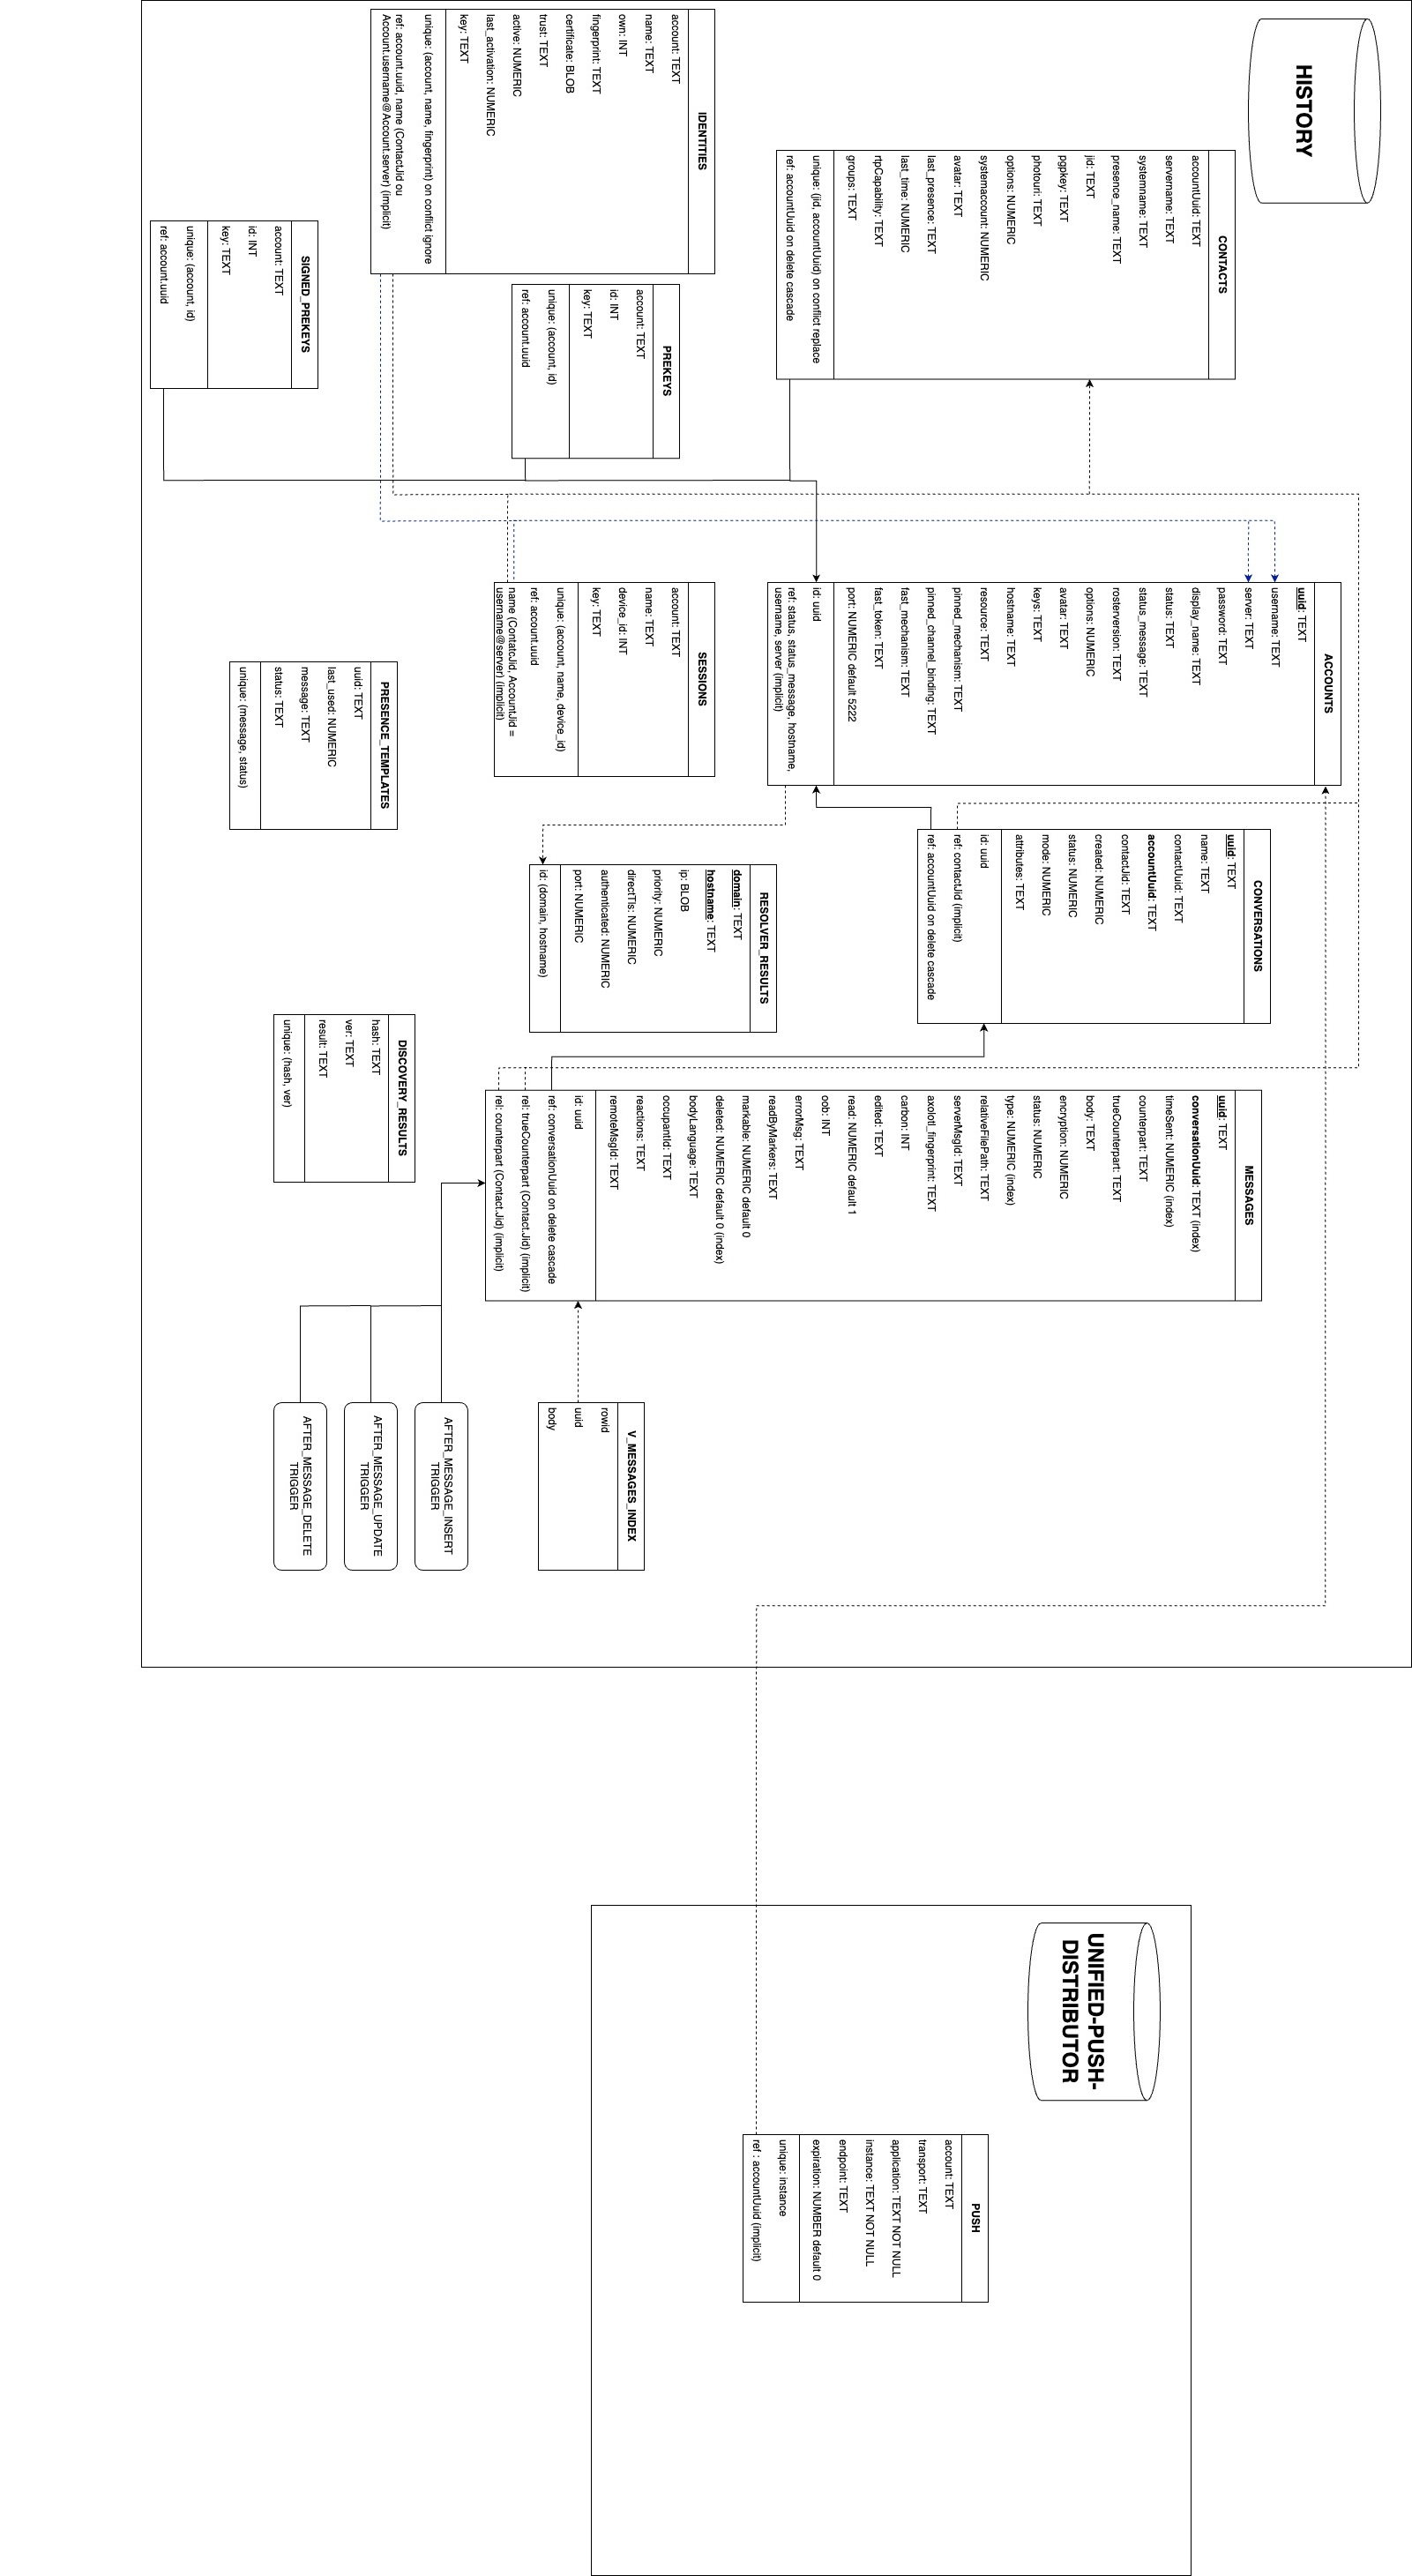
\includegraphics[scale=0.25]{Scema_Physique-Physique.jpg}
\end{center}

\section*{Statistics about the database queries}

\subsection*{Statistiques}

\subsubsection*{Métriques grâce à SQLInspect}

Grâce à l'outil \texttt{SQLInspect}, nous avons pu collecter les métriques suivantes sur les interactions SQL dans le projet, réparties par fichier :

\begin{itemize}
    \item \textbf{ImportBackupService.java} :
    \begin{itemize}
        \item \texttt{Queries} : 1
        \item \texttt{Inserts} : 0
        \item \texttt{Selects} : 1
        \item \texttt{Updates} : 0
        \item \texttt{Deletes} : 0
    \end{itemize}
    \item \textbf{DatabaseBackend.java} :
    \begin{itemize}
        \item \texttt{Queries} : 112
        \item \texttt{Inserts} : 1
        \item \texttt{Selects} : 10
        \item \texttt{Updates} : 8
        \item \texttt{Deletes} : 3
    \end{itemize}
    \item \textbf{UnifiedPushDatabase.java} :
    \begin{itemize}
        \item \texttt{Queries} : 2
        \item \texttt{Inserts} : 0
        \item \texttt{Selects} : 1
        \item \texttt{Updates} : 0
        \item \texttt{Deletes} : 0
    \end{itemize}
    \item \textbf{ExportBackupWorker.java} :
    \begin{itemize}
        \item \texttt{Queries} : 1
        \item \texttt{Inserts} : 0
        \item \texttt{Selects} : 1
        \item \texttt{Updates} : 0
        \item \texttt{Deletes} : 0
    \end{itemize}
\end{itemize}

\subsubsection*{Limitations de SQLInspect}

Bien que l'outil \texttt{SQLInspect} ait permis d'identifier une grande partie des interactions SQL dans le projet, il présente certaines limitations importantes. Notamment, \texttt{SQLInspect} n'est pas en mesure de reconstruire les requêtes SQL formées dynamiquement en Java à l'aide des méthodes \texttt{.query()}, \texttt{.insert()}, \texttt{.delete()} et \texttt{.update()}. Cela entraîne un sous-dénombrement des interactions SQL dans les fichiers analysés.

En analysant manuellement le code, nous avons pu identifier les requêtes SQL supplémentaires suivantes :

\begin{itemize}
    \item \textbf{DatabaseBackend.java} :
    \begin{itemize}
        \item \texttt{Insert} : 12 requêtes supplémentaires.
        \item \texttt{Select} : 21 requêtes supplémentaires.
        \item \texttt{Delete} : 15 requêtes supplémentaires.
        \item \texttt{Update} : 16 requêtes supplémentaires.
    \end{itemize}
    \item \textbf{UnifiedPushDatabase.java} :
    \begin{itemize}
        \item \texttt{Insert} : 1 requête supplémentaire.
        \item \texttt{Select} : 6 requêtes supplémentaires.
        \item \texttt{Delete} : 3 requêtes supplémentaires.
        \item \texttt{Update} : 1 requête supplémentaire.
    \end{itemize}
    \item \textbf{ImportBackupService.java} :
    \begin{itemize}
        \item \texttt{Insert} : 1 requête supplémentaire.
    \end{itemize}
    \item \textbf{ExportBackupWorker.java} :
    \begin{itemize}
        \item \texttt{Select} : 2 requêtes supplémentaires.
    \end{itemize}
\end{itemize}

\paragraph{Impact des limitations :}
Ces requêtes manquantes montrent que les résultats fournis par \texttt{SQLInspect} sous-estiment l'activité SQL réelle dans le projet. Cela met en évidence la nécessité de combiner les analyses automatiques avec une validation manuelle pour obtenir une image complète des interactions SQL.


Ces métriques fournissent une vue d'ensemble de l'activité SQL à travers les différents fichiers du projet et mettent en lumière les zones critiques, comme \textbf{DatabaseBackend.java}, qui contient la majorité des requêtes SQL.

\subsubsection*{Rôles des fichiers}

Chaque fichier analysé dans ce projet a un rôle spécifique en lien avec les interactions SQL et la gestion des données. Voici une description détaillée des responsabilités de chaque fichier :

\begin{itemize}
    \item \textbf{ImportBackupService.java} :
    \begin{itemize}
        \item Ce fichier est responsable de l'importation des données, notamment les informations liées à un compte utilisateur.
        \item Les requêtes SQL ici servent principalement à insérer ou récupérer des données importées pour les intégrer dans les tables appropriées.
    \end{itemize}

    \item \textbf{ExportBackupWorker.java} :
    \begin{itemize}
        \item Ce fichier gère l'exportation des informations d'un compte utilisateur.
        \item Les interactions SQL consistent principalement à extraire les données nécessaires pour créer un fichier de sauvegarde ou transférer les informations.
    \end{itemize}

    \item \textbf{UnifiedPushDatabase.java} :
    \begin{itemize}
        \item Ce fichier est chargé de la gestion des notifications push.
        \item Les requêtes SQL ici concernent principalement la gestion des endpoints, des tokens d'authentification et des informations liées aux notifications.
    \end{itemize}

    \item \textbf{DatabaseBackend.java} :
    \begin{itemize}
        \item Ce fichier contient la logique principale pour toutes les interactions SQL du projet.
        \item Il centralise les opérations complexes telles que l'insertion, la mise à jour, la suppression et la récupération des données.
        \item La majorité des requêtes SQL identifiées se trouvent dans ce fichier, ce qui en fait le cœur de la gestion des données dans l'application.
    \end{itemize}
\end{itemize}

\paragraph{Conclusion :}
Chaque fichier joue un rôle précis et complémentaire dans le projet. Cependant, la logique principale et la majorité des interactions SQL résident dans \textbf{DatabaseBackend.java}, qui sert de base à toutes les fonctionnalités de gestion des données.

\subsubsection*{Analyse de complexité des requêtes SQL}

Dans le fichier \texttt{DatabaseBackend.java}, les requêtes SQL identifiées présentent une complexité variable selon leur type et leur usage. Dans la plupart des cas, elles restent simples et intuitives. Voici une analyse détaillée, accompagnée d'exemples concrets tirés du code.

\begin{itemize}
    \item \textbf{INSERT} :
    \begin{itemize}
        \item La majorité des requêtes \texttt{INSERT} insèrent simplement des données sans complexité particulière. Exemple :
        \begin{lstlisting}[language=Java]
public void createMessage(Message message) {
    SQLiteDatabase db = this.getWritableDatabase();
    db.insert(Message.TABLENAME, null, message.getContentValues());
}
        \end{lstlisting}
        \item Quelques cas incluent une étape préalable, comme un \texttt{DELETE}, augmentant légèrement la complexité. Exemple :
        \begin{lstlisting}[language=Java]
public void insertPresenceTemplate(PresenceTemplate template) {
    SQLiteDatabase db = this.getWritableDatabase();
    db.delete(PresenceTemplate.TABELNAME, 
              PresenceTemplate.UUID + " not in (select " + 
              PresenceTemplate.UUID + " from " + 
              PresenceTemplate.TABELNAME + " order by " + 
              PresenceTemplate.LAST_USED + " desc limit 9)", null);
    db.insert(PresenceTemplate.TABELNAME, null, 
    template.getContentValues());
}
        \end{lstlisting}
    \end{itemize}
    
    \item \textbf{SELECT} :
    \begin{itemize}
        \item La plupart des \texttt{SELECT} récupèrent des données directement, sans jointures ni filtres complexes. Exemple :
        \begin{lstlisting}[language=Java]
public List<PresenceTemplate> getPresenceTemplates() {
    ArrayList<PresenceTemplate> templates = new ArrayList<>();
    SQLiteDatabase db = this.getReadableDatabase();
    Cursor cursor = db.query(PresenceTemplate.TABELNAME, 
                             null, null, null, null, null, 
                             PresenceTemplate.LAST_USED + " desc");
    while (cursor.moveToNext()) {
        templates.add(PresenceTemplate.fromCursor(cursor));
    }
    cursor.close();
    return templates;
}
        \end{lstlisting}
        \item Certains cas incluent des jointures complexes et des filtres avancés. Exemple :
        \begin{lstlisting}[language=Java]
public Cursor getMessageSearchCursor(final List<String> term,
final String uuid) {
    final SQLiteDatabase db = this.getReadableDatabase();
    final StringBuilder SQL = new StringBuilder();
    SQL.append("SELECT messages.*, conversations.contactJid, ")
       .append("conversations.account, conversations.mode ")
       .append("FROM messages JOIN conversations ON ")
       .append("messages.conversation = conversations.uuid ")
       .append("WHERE messages.body MATCH ?");
    if (uuid != null) {
        SQL.append(" AND conversations.uuid = ?");
    }
    return db.rawQuery(SQL.toString(), selectionArgs);
}
        \end{lstlisting}
    \end{itemize}
    
    \item \textbf{UPDATE} :
    \begin{itemize}
        \item Les requêtes \texttt{UPDATE} sont souvent conditionnelles, mais restent simples. Exemple :
        \begin{lstlisting}[language=Java]
public boolean updateMessage(final Message message, 
final boolean includeBody) {
    final var db = this.getWritableDatabase();
    final var contentValues = message.getContentValues();
    if (!includeBody) {
        contentValues.remove(Message.BODY);
    }
    return db.update(Message.TABLENAME, contentValues, 
                     Message.UUID + "=?", 
                     new String[]{message.getUuid()}) == 1;
}
        \end{lstlisting}
        \item Certains cas incluent des transactions, augmentant la complexité. Exemple :
        \begin{lstlisting}[language=Java]
public void markFilesAsChanged(List<FilePathInfo> files) {
    SQLiteDatabase db = this.getReadableDatabase();
    db.beginTransaction();
    for (FilePathInfo info : files) {
        ContentValues contentValues = new ContentValues();
        contentValues.put(Message.DELETED, info.deleted ? 1 : 0);
        db.update(Message.TABLENAME, contentValues, 
                  Message.UUID + "=?", 
                  new String[]{info.uuid.toString()});
    }
    db.setTransactionSuccessful();
    db.endTransaction();
}
        \end{lstlisting}
    \end{itemize}
    
    \item \textbf{DELETE} :
    \begin{itemize}
        \item Les \texttt{DELETE} sont majoritairement simples, basées sur des conditions uniques. Exemple :
        \begin{lstlisting}[language=Java]
public boolean deleteAccount(final Account account) {
    final var db = this.getWritableDatabase();
    return db.delete(Account.TABLENAME, 
                     Account.UUID + "=?", 
                     new String[]{account.getUuid()}) == 1;
}
        \end{lstlisting}
        \item Quelques cas incluent des conditions multiples. Exemple :
        \begin{lstlisting}[language=Java]
public void deleteAllSessions(Account account, 
SignalProtocolAddress contact) {
    SQLiteDatabase db = this.getWritableDatabase();
    String[] args = {account.getUuid(), contact.getName()};
    db.delete(SQLiteAxolotlStore.SESSION_TABLENAME, 
              SQLiteAxolotlStore.ACCOUNT + "=? AND " + 
              SQLiteAxolotlStore.NAME + " = ?", args);
}
        \end{lstlisting}
    \end{itemize}
\end{itemize}

\paragraph{Conclusion :}
Dans l'ensemble, les requêtes SQL du fichier \texttt{DatabaseBackend.java} sont \textbf{simples et intuitives} à comprendre. Les scénarios complexes, tels que les transactions ou les jointures, restent cohérents et logiques.

\texttt{SQLInspect} offre une analyse utile de la complexité, notamment en identifiant les imbrications dans les requêtes. Cependant, il ne capture pas la majorité des requêtes dynamiques (comme celles formées par \texttt{.query()}, \texttt{.insert()}, \texttt{.update()}, ou \texttt{.delete()}), ce qui limite son utilité pour ces types de requêtes qui dominent notre code.

\subsection*{Sous-schéma logique}

Pour répondre à la question visant à dériver le Logical SubSchema (LSS), il est nécessaire d’identifier les éléments du schéma (tables et colonnes) réellement exploités par les programmes. Le LSS est obtenu en excluant toutes les parties inutilisées du schéma logique initial (LS), de manière à refléter uniquement les interactions effectives entre le code source et la base de données.

La méthodologie suivie pour cette analyse est la suivante :
\begin{enumerate}
    \item Identifier toutes les tables définies dans le schéma logique initial (LS).
    \item Pour chaque table, examiner le code source afin de localiser toutes les interactions, en particulier :
    \item Les opérations utilisant des curseurs (\texttt{Cursor}) pour extraire des colonnes spécifiques via des méthodes telles que \texttt{getColumnIndexOrThrow}.
    \item Analyser les méthodes associées aux curseurs et aux requêtes pour déterminer où elles sont appelées dans le programme, et identifier les colonnes réellement utilisées pour chaque table.
    \item Construire le Logical SubSchema (LSS) en conservant uniquement les tables et colonnes utilisées par le programme.
\end{enumerate}

Cette approche garantit une vue précise des éléments du schéma qui sont essentiels au fonctionnement du programme, tout en éliminant les parties redondantes ou inutilisées. 
Il est important de noter que, bien que les méthodes comme \texttt{.query()} insèrent majoritairement toutes les colonnes d'une table dans le curseur ( \texttt{SELECT *}) dans notre programme, nous avons pris le parti de ne pas simplement considérer ces colonnes comme utilisées. Une vérification plus approfondie a été effectuée pour déterminer si les colonnes récupérées dans les curseurs sont réellement exploitées dans le programme. Cela garantit que le LSS reflète uniquement les interactions effectives et significatives entre le code source et la base de données.


\subsubsection*{Table Account}

La classe \texttt{Account} utilise toutes les colonnes de la table \texttt{Account} dans la méthode \texttt{Account.fromCursor(Cursor cursor)}. Les colonnes suivantes sont utilisées :

\begin{itemize}
    \item \texttt{UUID}
    \item \texttt{USERNAME}
    \item \texttt{SERVER}
    \item \texttt{PASSWORD}
    \item \texttt{OPTIONS}
    \item \texttt{ROSTERVERSION}
    \item \texttt{KEYS}
    \item \texttt{AVATAR}
    \item \texttt{DISPLAY\_NAME}
    \item \texttt{HOSTNAME}
    \item \texttt{PORT}
    \item \texttt{STATUS}
    \item \texttt{STATUS\_MESSAGE}
    \item \texttt{RESOURCE}
    \item \texttt{PINNED\_MECHANISM}
    \item \texttt{PINNED\_CHANNEL\_BINDING}
    \item \texttt{FAST\_MECHANISM}
    \item \texttt{FAST\_TOKEN}
\end{itemize}

Ainsi, la méthode \texttt{fromCursor} garantit une couverture complète des colonnes de la table \texttt{Account}.

\subsubsection*{Table Contact}

La classe \texttt{Contact} utilise toutes les colonnes de la table \texttt{Contact} dans la méthode \texttt{Contact.fromCursor(Cursor cursor)}. Les colonnes suivantes sont utilisées :

\begin{itemize}
    \item \texttt{ACCOUNT}
    \item \texttt{SYSTEMNAME}
    \item \texttt{SERVERNAME}
    \item \texttt{PRESENCE\_NAME}
    \item \texttt{JID}
    \item \texttt{OPTIONS}
    \item \texttt{SYSTEMACCOUNT}
    \item \texttt{PHOTOURI}
    \item \texttt{KEYS}
    \item \texttt{AVATAR}
    \item \texttt{LAST\_PRESENCE}
    \item \texttt{LAST\_TIME}
    \item \texttt{GROUPS}
    \item \texttt{RTP\_CAPABILITY}
\end{itemize}

Ainsi, la méthode \texttt{fromCursor} garantit une couverture complète des colonnes de la table \texttt{Contact}.

\subsubsection*{Table Conversation}

La classe \texttt{Conversation} utilise toutes les colonnes de la table \texttt{Conversation} dans la méthode \texttt{Conversation.fromCursor(Cursor cursor)}. Les colonnes suivantes sont utilisées :

\begin{itemize}
    \item \texttt{UUID}
    \item \texttt{NAME}
    \item \texttt{CONTACT}
    \item \texttt{ACCOUNT}
    \item \texttt{CONTACTJID}
    \item \texttt{CREATED}
    \item \texttt{STATUS}
    \item \texttt{MODE}
    \item \texttt{ATTRIBUTES}
\end{itemize}

Ainsi, la méthode \texttt{fromCursor} garantit une couverture complète des colonnes de la table \texttt{Conversation}.

\subsubsection*{Table PresenceTemplate}

La classe \texttt{PresenceTemplate} utilise toutes les colonnes de la table \texttt{PresenceTemplate} dans la méthode \texttt{PresenceTemplate.fromCursor(Cursor cursor)}. Les colonnes suivantes sont utilisées :

\begin{itemize}
    \item \texttt{UUID}
    \item \texttt{MESSAGE}
    \item \texttt{STATUS}
\end{itemize}

Ainsi, la méthode \texttt{fromCursor} garantit une couverture complète des colonnes de la table \texttt{PresenceTemplate} sauf pour \texttt{last\_used} car la variable capturant cette colonne est private et n'est donc pas utilisable dans le code et il n'y a pas de getter ni setter pour cette variable.


\subsubsection*{Table Message}

La classe \texttt{Message} utilise toutes les colonnes de la table \texttt{Message} dans la méthode \texttt{Message.fromCursor(Cursor cursor, Conversation conversation)}. Les colonnes suivantes sont utilisées :

\begin{itemize}
    \item \texttt{UUID}
    \item \texttt{CONVERSATION}
    \item \texttt{COUNTERPART}
    \item \texttt{TRUE\_COUNTERPART}
    \item \texttt{BODY}
    \item \texttt{TIME\_SENT}
    \item \texttt{ENCRYPTION}
    \item \texttt{STATUS}
    \item \texttt{TYPE}
    \item \texttt{CARBON}
    \item \texttt{REMOTE\_MSG\_ID}
    \item \texttt{RELATIVE\_FILE\_PATH}
    \item \texttt{SERVER\_MSG\_ID}
    \item \texttt{FINGERPRINT}
    \item \texttt{READ}
    \item \texttt{EDITED}
    \item \texttt{OOB}
    \item \texttt{ERROR\_MESSAGE}
    \item \texttt{READ\_BY\_MARKERS}
    \item \texttt{MARKABLE}
    \item \texttt{DELETED}
    \item \texttt{BODY\_LANGUAGE}
    \item \texttt{OCCUPANT\_ID}
    \item \texttt{REACTIONS}
\end{itemize}

Ainsi, la méthode \texttt{fromCursor} garantit une couverture complète des colonnes de la table \texttt{Message}.

\subsubsection*{Tables prekeys et signed\_prekeys}

Les classes utilisant les tables \texttt{prekeys} et \texttt{signed\_prekeys} garantissent une couverture des colonnes suivantes :

\paragraph{Table prekeys}
Les colonnes de la table \texttt{prekeys} sont utilisées dans les méthodes associées au \texttt{PreKeyStore} :
\begin{itemize}
    \item \texttt{ACCOUNT} : Identifiant de l'utilisateur associé à la clé.
    \item \texttt{ID} : Identifiant unique de la clé.
    \item \texttt{KEY} : Valeur de la clé prépartagée.
\end{itemize}

Méthodes impliquées dans l'accès à la table \texttt{prekeys} :
\begin{itemize}
    \item \texttt{SQLiteAxolotlStore.loadPreKey(int preKeyId)} : Charge un enregistrement de clé prépartagée.
    \item \texttt{SQLiteAxolotlStore.storePreKey(int preKeyId, PreKeyRecord record)} : Stocke un enregistrement de clé prépartagée.
    \item \texttt{SQLiteAxolotlStore.containsPreKey(int preKeyId)} : Vérifie l'existence d'une clé prépartagée.
    \item \texttt{SQLiteAxolotlStore.removePreKey(int preKeyId)} : Supprime une clé prépartagée.
    \item \texttt{SQLiteAxolotlStore.flushPreKeys()} : Supprime les clés marquées pour suppression.
\end{itemize}

\paragraph{Table signed\_prekeys}
Les colonnes de la table \texttt{signed\_prekeys} sont utilisées dans les méthodes associées au \texttt{SignedPreKeyStore} :
\begin{itemize}
    \item \texttt{ACCOUNT} : Identifiant de l'utilisateur associé à la clé.
    \item \texttt{ID} : Identifiant unique de la clé signée.
    \item \texttt{KEY} : Valeur de la clé signée.
\end{itemize}

Méthodes impliquées dans l'accès à la table \texttt{signed\_prekeys} :
\begin{itemize}
    \item \texttt{SQLiteAxolotlStore.loadSignedPreKey(int signedPreKeyId)} : Charge un enregistrement de clé signée.
    \item \texttt{SQLiteAxolotlStore.storeSignedPreKey(int signedPreKeyId, SignedPreKeyRecord record)} : Stocke un enregistrement de clé signée.
    \item \texttt{SQLiteAxolotlStore.containsSignedPreKey(int signedPreKeyId)} : Vérifie l'existence d'une clé signée.
    \item \texttt{SQLiteAxolotlStore.removeSignedPreKey(int signedPreKeyId)} : Supprime une clé signée.
    \item \texttt{SQLiteAxolotlStore.loadSignedPreKeys()} : Charge toutes les clés signées.
\end{itemize}

\subsubsection*{Table identities}

La table \texttt{identities} est utilisée pour stocker et gérer les identités Signal Protocol. Les colonnes définies dans cette table sont les suivantes :

\begin{itemize}
    \item \texttt{ACCOUNT} : Identifiant de l'utilisateur associé.
    \item \texttt{NAME} : Nom associé à l'identité.
    \item \texttt{OWN} : Indicateur si l'identité appartient à l'utilisateur local.
    \item \texttt{FINGERPRINT} : Empreinte unique de la clé d'identité.
    \item \texttt{CERTIFICATE} : Certificat X509 associé.
    \item \texttt{TRUST} : Niveau de confiance pour cette identité.
    \item \texttt{ACTIVE} : Indicateur si l'identité est active.
    \item \texttt{LAST\_ACTIVATION} : Dernière date d'activation de l'identité.
    \item \texttt{KEY} : Valeur de la clé publique associée.
\end{itemize}

\paragraph{Utilisation des colonnes via un curseur :}
\begin{itemize}
    \item \textbf{Méthode \texttt{FingerprintStatus.fromCursor(Cursor cursor)}} :
    \begin{itemize}
        \item Colonnes utilisées : \texttt{TRUST}, \texttt{ACTIVE}, \texttt{LAST\_ACTIVATION}.
    \end{itemize}
    \item \textbf{Méthode \texttt{getFingerprintStatus}} :
    \begin{itemize}
        \item Colonnes utilisées : \texttt{FINGERPRINT}, \texttt{TRUST}.
    \end{itemize}
    \item \textbf{Méthode \texttt{setFingerprintStatus}} :
    \begin{itemize}
        \item Colonnes utilisées : \texttt{FINGERPRINT}, \texttt{TRUST}, \texttt{ACTIVE}.
    \end{itemize}
    \item \textbf{Méthode \texttt{setFingerprintCertificate}} :
    \begin{itemize}
        \item Colonnes utilisées : \texttt{FINGERPRINT}, \texttt{CERTIFICATE}.
    \end{itemize}
    \item \textbf{Méthode \texttt{loadIdentityKeys}} :
    \begin{itemize}
        \item Colonnes utilisées : \texttt{ACCOUNT}, \texttt{NAME}, \texttt{FINGERPRINT}, \texttt{TRUST}, \texttt{OWN}, \texttt{KEY}.
    \end{itemize}
    \item \textbf{Méthode \texttt{storeIdentityKey}} :
    \begin{itemize}
        \item Colonnes utilisées : \texttt{ACCOUNT}, \texttt{NAME}, \texttt{FINGERPRINT}, \texttt{TRUST}.
    \end{itemize}
\end{itemize}

\paragraph{Colonnes non utilisées :}
\begin{itemize}
    Toutes les colonnes sont utilisées.
\end{itemize}

\subsubsection*{Table sessions}

La table \texttt{sessions} est utilisée pour gérer les sessions Signal Protocol. Les colonnes définies dans cette table sont les suivantes :

\begin{itemize}
    \item \texttt{ACCOUNT} : Identifiant de l'utilisateur associé à la session.
    \item \texttt{NAME} : Nom du correspondant.
    \item \texttt{DEVICE\_ID} : Identifiant unique du périphérique.
    \item \texttt{KEY} : Données de la session.
\end{itemize}

\paragraph{Utilisation des colonnes via un curseur :}
\begin{itemize}
    \item \textbf{Méthode \texttt{loadSession}} :
    \begin{itemize}
        \item Colonnes utilisées : \texttt{ACCOUNT}, \texttt{NAME}, \texttt{DEVICE\_ID}, \texttt{KEY}.
    \end{itemize}
    \item \textbf{Méthode \texttt{storeSession}} :
    \begin{itemize}
        \item Colonnes utilisées : \texttt{ACCOUNT}, \texttt{NAME}, \texttt{DEVICE\_ID}, \texttt{KEY}.
    \end{itemize}
    \item \textbf{Méthode \texttt{containsSession}} :
    \begin{itemize}
        \item Colonnes utilisées : \texttt{ACCOUNT}, \texttt{NAME}, \texttt{DEVICE\_ID}.
    \end{itemize}
    \item \textbf{Méthode \texttt{deleteSession}} :
    \begin{itemize}
        \item Colonnes utilisées : \texttt{ACCOUNT}, \texttt{NAME}, \texttt{DEVICE\_ID}.
    \end{itemize}
\end{itemize}

\paragraph{Colonnes non utilisées :}
\begin{itemize}
    \item Toutes les colonnes sont utilisées.
\end{itemize}

\subsubsection*{Table PUSH}

La table \texttt{PUSH} est utilisée pour gérer les notifications push dans l'application. Les colonnes définies dans cette table sont les suivantes :

\begin{itemize}
    \item \texttt{account} : Identifiant de l'utilisateur associé.
    \item \texttt{transport} : Type de transport utilisé pour la notification push.
    \item \texttt{application} : Nom de l'application.
    \item \texttt{instance} : Instance unique (valeur unique dans la table).
    \item \texttt{endpoint} : URL de l'endpoint pour la notification push.
    \item \texttt{expiration} : Timestamp de l'expiration de l'entrée.
\end{itemize}

\paragraph{Utilisation des colonnes via un curseur :}
\begin{itemize}
    \item \textbf{Méthode \texttt{register}} :
    \begin{itemize}
        \item Colonnes utilisées : \texttt{application}, \texttt{instance}.
    \end{itemize}
    \item \textbf{Méthode \texttt{getRenewals}} :
    \begin{itemize}
        \item Colonnes utilisées : \texttt{application}, \texttt{instance}, \texttt{account}, \texttt{transport}, \texttt{expiration}.
    \end{itemize}
    \item \textbf{Méthode \texttt{getEndpoint}} :
    \begin{itemize}
        \item Colonnes utilisées : \texttt{account}, \texttt{transport}, \texttt{instance}, \texttt{endpoint}, \texttt{expiration}.
    \end{itemize}
    \item \textbf{Méthode \texttt{deletePushTargets}} :
    \begin{itemize}
        \item Colonnes utilisées : \texttt{application}, \texttt{instance}.
    \end{itemize}
    \item \textbf{Méthode \texttt{hasEndpoints}} :
    \begin{itemize}
        \item Colonnes utilisées : \texttt{endpoint}.
    \end{itemize}
    \item \textbf{Méthode \texttt{updateEndpoint}} :
    \begin{itemize}
        \item Colonnes utilisées : \texttt{instance}, \texttt{account}, \texttt{transport}, \texttt{endpoint}, \texttt{expiration}.
    \end{itemize}
    \item \textbf{Méthode \texttt{getPushTargets}} :
    \begin{itemize}
        \item Colonnes utilisées : \texttt{application}, \texttt{instance}, \texttt{account}.
    \end{itemize}
    \item \textbf{Méthode \texttt{deleteInstance}} :
    \begin{itemize}
        \item Colonnes utilisées : \texttt{instance}.
    \end{itemize}
    \item \textbf{Méthode \texttt{deleteApplication}} :
    \begin{itemize}
        \item Colonnes utilisées : \texttt{application}.
    \end{itemize}
\end{itemize}

\paragraph{Colonnes non utilisées :}
\begin{itemize}
    \item Toutes les colonnes définies sont utilisées.
\end{itemize}

\subsubsection*{Table Discovery Results}

La table \texttt{discovery\_results} est utilisée pour stocker les résultats de découverte de services. Les colonnes définies dans cette table sont les suivantes :

\begin{itemize}
    \item \texttt{HASH} : Hachage unique associé au résultat de découverte.
    \item \texttt{VER} : Version ou identifiant du résultat.
    \item \texttt{RESULT} : Résultat de la découverte, stocké en tant que chaîne JSON.
\end{itemize}

\paragraph{Utilisation des colonnes via un curseur :}
\begin{itemize}
    \item \textbf{Méthode \texttt{ServiceDiscoveryResult(Cursor cursor)}} :
    \begin{itemize}
        \item Colonnes utilisées : \texttt{HASH}, \texttt{VER}, \texttt{RESULT}.
    \end{itemize}
\end{itemize}

\paragraph{Colonnes non utilisées :}
\begin{itemize}
    \item Toutes les colonnes définies sont utilisées.
\end{itemize}

\subsubsection*{Table Resolver Results}

La table \texttt{resolver\_results} est utilisée pour stocker les résultats de résolution DNS. Les colonnes définies dans cette table sont les suivantes :

\begin{itemize}
    \item \texttt{DOMAIN} : Domaine pour lequel la résolution est effectuée.
    \item \texttt{HOSTNAME} : Nom d'hôte obtenu pour le domaine.
    \item \texttt{IP} : Adresse IP correspondante.
    \item \texttt{PRIORITY} : Priorité du résultat.
    \item \texttt{DIRECT\_TLS} : Indique si TLS direct est activé.
    \item \texttt{AUTHENTICATED} : Indique si la connexion est authentifiée.
    \item \texttt{PORT} : Port associé à la connexion.
\end{itemize}

\paragraph{Utilisation des colonnes via un curseur :}
\begin{itemize}
    \item \textbf{Méthode \texttt{findResolverResult}} :
    \begin{itemize}
        \item Colonnes utilisées : \texttt{DOMAIN}, \texttt{HOSTNAME}, \texttt{IP}, \texttt{PRIORITY}, \texttt{DIRECT\_TLS}, \texttt{AUTHENTICATED}, \texttt{PORT}.
        \item Cette méthode est utilisée dans le fichier \texttt{XmppConnection.java}.
    \end{itemize}
    \item \textbf{Méthode \texttt{saveResolverResult}} :
    \begin{itemize}
        \item Colonnes utilisées : \texttt{DOMAIN}, \texttt{HOSTNAME}, \texttt{IP}, \texttt{PRIORITY}, \texttt{DIRECT\_TLS}, \texttt{AUTHENTICATED}, \texttt{PORT}.
        \item Cette méthode est utilisée dans le fichier \texttt{XmppConnection.java}.
    \end{itemize}
\end{itemize}

\paragraph{Colonnes non utilisées :}
\begin{itemize}
    \item Toutes les colonnes définies sont utilisées.
\end{itemize}

\paragraph{Conclusion :}

Après une analyse approfondie du code on a montré que toutes les colonnes et tables sont utilisées dans le code sauf \texttt{PresenceTemplate.last\_used}.


\section*{Étape 3 : Analyse « What-If » et Scénarios d'Évolution}

\subsection*{Introduction}
Dans cette étape, nous appliquons une analyse « what-if » pour évaluer l'impact de 10 scénarios d'évolution sur le Sous-Schéma Physique (PSS) de notre système de base de données. Chaque scénario est accompagné d'une description détaillée et de son impact sur le code source, incluant les classes, méthodes, et requêtes SQL affectées.

\subsection*{Scénario 1 : Ajout de contrainte dans le moteur de base de données}

\subsubsection*{Résumé du changement :}

Lors de notre analyse du code Java et DDL de l'application, nous avons remarqué que certaines colonnes dans les tables de la base de données peuvent contenir des valeurs nulles et d'autres ne sont plus utilisées . Cependant, le code Java ne semble pas gérer ces valeurs nulles. Pour éviter des erreurs potentielles, nous allons ajouter des contraintes \textit{NOT NULL} sur ces colonnes.

\subsubsection*{Détail des changements :}

\paragraph{Colonnes à modifier :}
\begin{itemize}
	\item Dans la table \texttt{contacts}, la colonne \texttt{jid} peut être \texttt{NULL}. Nous allons ajouter une contrainte \texttt{NOT NULL} pour garantir que chaque contact a un identifiant Jabber valide.
	\item Dans la table \texttt{accounts}, les colonnes \texttt{username} et \texttt{server} peuvent être \texttt{NULL}. Nous allons ajouter une contrainte \texttt{NOT NULL} pour garantir que chaque compte possède un server et un username. Ce qui revient à dire que chaque compte doit avoir un identifiant Jabber valide.
	\item Dans la table \texttt{conversation}, la colonne \texttt{contactUuid} ne semble plus réutilisée car ne référence pas une colonne \texttt{uuid} dans la table \texttt{contact}. Nous allons supprimer cette colonne. La colonne \texttt{contactJid} ne dois aussi pas être null. De plus, cette colonne et la colonne \texttt{contactUuid} doivent être unique. 
\end{itemize}

Il est  quand même sage de vérifier que les colonnes à modifier ne contiennent pas de valeurs nulles avant d'appliquer les contraintes \texttt{NOT NULL}.

Par simplicité, nous allons supprimer les instances qui possèdent des valeurs nulles pour les colonnes où on ajoute la contrainte \texttt{NOT NULL}. Mais il faudrait faire un backup de la base de données avant d'appliquer ces changements.

\begin{lstlisting}[language=SQL]
DELETE FROM contacts WHERE jid IS NULL;
ALTER TABLE contacts ALTER COLUMN jid SET NOT NULL;

DELETE FROM accounts WHERE username IS NULL OR server IS NULL;
ALTER TABLE accounts ALTER COLUMN username SET NOT NULL;
ALTER TABLE accounts ALTER COLUMN server SET NOT NULL;

DELETE FROM conversation WHERE jid IS NULL;
ALTER TABLE conversation DROP COLUMN contactUuid;
ALTER TABLE conversation ALTER COLUMN contactJid SET NOT NULL;
ALTER TABLE conversation ADD UNIQUE(contactJid, accountUuid)
 ON CONFLICT IGNORE;
\end{lstlisting}

Il est maintenant possible de déclarer explicitement la clé étrangère \texttt{contactJid} dans la table \texttt{Conversation}.

\begin{lstlisting}[language=SQL]
ALTER TABLE conversation ADD FOREIGN KEY(contactJid) 
 REFERENCES contact(jid) ON DELETE CASCADE;
\end{lstlisting}

On notera que dans la classe \texttt{Contact}, seule la colonne \texttt{jid} profite de l'ajout de la contrainte \texttt{NOT NULL}. La colonne \texttt{accountUuid} n'en profite pas, car cela ne poserait pas de problème avec le code actuel de l'application. Malgré tout, il est nécessaire d'avoir à la fois un \texttt{jid} et un \texttt{accountUuid} pour identifier un contact.

\subsubsection*{Impact sur le code :}

L'idée de ce scénario est de s'assurer que les colonnes qui ne doivent pas être \texttt{NULL} ne le sont pas. Le code Java ne va pas être directement impacté par ces changements. Mais il faut tout de même faire tourner les tests pour s'assurer que l'application fonctionne toujours correctement.

\subsubsection*{Test à effectuer :}

\begin{itemize}
	\item Vérifier que les colonnes modifiées ne contiennent pas de valeurs nulles.
	\item Appliquer les contraintes \texttt{NOT NULL} et vérifier que les valeurs nulles sont supprimées.
	\item Tester les fonctionnalités principales de l'application pour s'assurer qu'elles fonctionnent toujours correctement.
\end{itemize}

\subsection*{Scénario 2 : Ajout d'une fonctionnalité d'appel}

\subsubsection*{Résumé du changement :}

Le protocole XMPP vient de se mettre à jour et permet maintenant de gérer des appels. Nous allons ajouter une fonctionnalité d'appel à l'application, en utilisant les fonctionnalités de base de l'application pour gérer les appels.

\subsubsection*{Détail des changements :}

\subsubsection*{Stratégie d'implémentation :}

La majorité des modifications nécessaires est liée au code Java. La base de données doit s'adapter à ces changements. Ici, nous sommes dans un scénario imaginaire, mais on peut imaginer qu'il faut ajouter une table \texttt{calls} pour stocker les informations sur les appels. Cette table contiendrait des informations sur le temps de début et de fin de l'appel, la durée, etc. Elle sera en relation avec la table conversation, ce qui permet de minimiser la quantité de données à stocker et de faciliter les requêtes.

Mais aussi de nouvelles colonnes techniques permettant d'effectuer des appels dans les tables \texttt{Account} et \texttt{Contact}. Par exemple, une colonne \texttt{voiceSecurityKey} dans la table \texttt{Account} pour stocker le mécanisme de chiffrement utilisé pour les appels. 

\subsubsection*{Modification :}

Dans un premier temps , nous allons ajouter une table \texttt{calls} pour stocker les informations sur les appels.

\begin{lstlisting}[language=SQL]
CREATE TABLE Calls (
	uuid TEXT PRIMARY KEY,
	conversationUuid TEXT,
	startTime NUMBER,
	duration NUMBER,
	status NUMBER,

	FOREIGN KEY(conversationUuid) 
	 REFERENCES conversation(uuid) ON DELETE CASCADE
);
\end{lstlisting}

Ensuite, nous allons ajouter des colonnes dans les tables \texttt{Account} et \texttt{Contact} pour stocker les informations nécessaires pour les appels.

\begin{lstlisting}[language=SQL]
ALTER TABLE accounts ADD COLUMN voiceSecurityKey TEXT;
ALTER TABLE contacts ADD COLUMN voiceSecurityKey TEXT;
\end{lstlisting}

\subsubsection*{Impact sur le code :}

L'ajout d'une telle fonctionnalité nécessite des modifications importantes dans le code Java. Il faudra ajouter des classes, des méthodes, des requêtes SQL, etc. pour gérer les appels. Il faudra aussi mettre à jour l'interface utilisateur pour permettre aux utilisateurs de passer des appels.

Voici une liste non exhaustive des modifications à apporter dans le code Java :
\begin{itemize}
	\item Ajout d'un package, ou tout du moins d'une classe, contenant la logique pour gérer les appels.
	\begin{itemize}
		\item Possibilité d'ajouter des appels à la base de données à la fin de l'appel. 
		\item Permettre de démarrer et de terminer un appel.
		\item Lister l'historique des appels. Exemple en utilisant des jointures mais bien sur, on préférera l'utilisation de l'ORM:\\
			\texttt{SELECT Calls.*, Contacts.presence\_name FROM Calls}\\
			\texttt{JOIN Conversation ON Calls.conversationUuid = Conversation.uuid}\\
			\texttt{JOIN Accounts ON Conversation.accountUuid = Accounts.uuid}\\
			\texttt{JOIN Contacts ON Conversation.contactJid = Contacts.jid}\\
			\texttt{AND Conversation.accountUuid = Contacts.accountUuid}\\
			\texttt{WHERE Accounts.uuid = 'target\_account\_uuid';}
	\end{itemize}
	\item Ajout d'un nouveau statut possible pour définir un template de présence. Celui-ci pourrait être \texttt{in-call}.
	\item Mise à jour de l'interface utilisateur pour permettre aux utilisateurs de passer des appels.
\end{itemize}

\subsubsection*{Test à effectuer :}

\begin{itemize}
	\item Faire des tests unitaires pour s'assurer que les appels sont correctement ajoutés à la base de données.
	\begin{itemize}
		\item Que ce passerai t-il si l'appel n'a pas de conversation associée (valeur Null).
		\item Que ce passerai t-il si aucune clé de sécurité a été définie pour l'appel.
		\item Ajout et suppression d'appel.
	\end{itemize}
	\item Tester les fonctionnalités d'appel pour s'assurer qu'elles fonctionnent correctement.
\end{itemize}

\subsection*{Scénario 3 : Ajout de la possibilité de lier un numéro de téléphone à un contact}

\subsubsection*{Résumé du changement :}

XMPP s'unifie avec les protocoles de messagerie traditionnels et permet maintenant d'envoyer des messages SMS et d'appeler des numéros de téléphone. Le numéro de téléphone remplace le \textit{jid}, il n'est donc plus question de \textit{jid} dans XMPP.

Nous allons ajouter la possibilité de lier un numéro de téléphone à un contact dans l'application. Et remplacer le \textit{jid} par le numéro de téléphone dans les tables \texttt{contacts} et \texttt{Account}.

Dans ce scénario, nous allons ignorer que certains contacts peuvent être des groupes, et donc ne pas avoir de numéro de téléphone.

\subsubsection*{Détail des changements :}

\subsubsection*{Stratégie d'implémentation :}

Dans le cas de la table \texttt{Account}, il est possible de remplacer le \textit{jid} par le numéro de téléphone. Cependant, dans les tables \texttt{Contacts}, le jid est utilisé comme pour une relation avec la table \texttt{Conversation} et \texttt{Message}. Il faudra donc modifier adéquatement les tables \texttt{Conversation} et \texttt{Message} pour utiliser le numéro de téléphone à la place du \textit{jid}.

Pour le code Java, une solution permettant de ne pas modifier le code en profondeur est possible dans le cas où le \texttt{jid} est simplement remplacé par le numéro de téléphone. On peut ajouter une méthode dans l'ORM permettant de récupérer les numéros de téléphone dans les différentes classes, tout en gardant les méthodes \texttt{getJid} qui serai un alias de \texttt{getPhoneNumber}. On devra, malgré tout, marquer le \texttt{getJid} comme \texttt{deprecated} afin éviter des erreurs dans le futur.

\subsubsection*{Modification :}

Dans un premiers temps nous allons ajouter le numéro de téléphone dans les tables \texttt{Account} et \texttt{Contacts}.

\begin{lstlisting}[language=SQL]
	ALTER TABLE accounts ADD COLUMN phoneNumber TEXT;
	ALTER TABLE contacts ADD COLUMN phoneNumber TEXT;
\end{lstlisting}

Ensuite, il faudra attendre que l'utilisateur ajoute les numéro de téléphone, aussi bien le sien que celui de ses contacts. 

Dès que cela est fait, il faudra aussi modifier les tables \texttt{Conversation} et \texttt{Message} pour utiliser le numéro de téléphone à la place du \textit{jid}.

Pour la table \texttt{Conversation} :

\begin{lstlisting}[language=SQL]
ALTER TABLE conversation 
ADD COLUMN contactPhoneNumber TEXT;

UPDATE conversation 
SET contactPhoneNumber = (
	SELECT phoneNumber FROM contacts 
	WHERE jid = contactJid
);

ALTER TABLE conversation DROP COLUMN contactJid;

ALTER TABLE conversation 
ADD UNIQUE(contactPhoneNumber, accountUuid)
ON CONFLICT IGNORE;
\end{lstlisting}

Et pour la table \texttt{Message} :

\begin{lstlisting}[language=SQL]
UPDATE message
WHERE trueCounterpart IS NOT NULL
SET trueCounterpart = (
	SELECT phoneNumber FROM contacts 
	WHERE jid = trueCounterpart
);

UPDATE message
WHERE counterpart IS NOT NULL
SET counterpart = (
	SELECT phoneNumber FROM contacts 
	WHERE jid = counterpart
);
\end{lstlisting}

\subsubsection*{Impact sur le code :}

L'impact sur le code Java est relativement faible, car il suffit de remplacer le \textit{jid} par le numéro de téléphone dans les classes qui manipulent les contacts. Il faudra aussi mettre à jour l'interface utilisateur pour permettre aux utilisateurs de saisir et de gérer les numéros de téléphone.

Il faudra aussi concevoir un script permettant à l'utilisateur de migrer ses contacts de \textit{jid} à numéro de téléphone, et puis lancer les requêtes SQL pour effectuer la migration.

\subsection*{Scénario 4 : Préférence de compte}

\subsubsection*{Résumé du changement :}

Nous allons ajouter une fonctionnalité de préférence de compte à l'application. Cela permettra aux utilisateurs de définir des préférences pour chaque compte, telles que le thème, la langue, etc.

\subsubsection*{Détail des changements :}

\subsubsection*{Stratégie d'implémentation :}

Pour ajouter cette fonctionnalité, nous allons ajouter une nouvelle table \texttt{accountPreferences} pour stocker les préférences de compte. Cette table sera en relation avec la table \texttt{Account}. Cela permettra à l'utilisateur de sauvegarder des configurations de préférences pour un même compte.

\subsubsection*{Modification :}

Nous allons ajouter une table \texttt{preferences} pour stocker les préférences de compte. Cette table sera en relation avec la table \texttt{Account}.

\begin{lstlisting}[language=SQL]
CREATE TABLE accountPreferences (
	uuid TEXT PRIMARY KEY,
	accountUuid TEXT,
	theme TEXT,
	language TEXT,
	FOREIGN KEY(accountUuid) 
	REFERENCES accounts(uuid) ON DELETE CASCADE
);
\end{lstlisting}

\subsubsection*{Impact sur le code :}

La plupart des modifications nécessaires pour ajouter cette fonctionnalité seront dans le code Java. Il faudra ajouter des classes, des méthodes, des requêtes SQL, etc. pour gérer les préférences de compte. Il faudra aussi mettre à jour l'interface utilisateur pour permettre aux utilisateurs de définir et de gérer leurs préférences.

Il faudra certainement utiliser des outils d'internationalisation pour gérer les préférences de langue.

\subsection*{Scénario 5 : Possibilité de contacter une intelligence artificielle}

\subsubsection*{Résumé du changement :}

Nous allons ajouter une fonctionnalité permettant aux utilisateurs de contacter une intelligence artificielle. Cela permettra aux utilisateurs de poser des questions à l'intelligence artificielle et de recevoir des réponses.

\subsubsection*{Détail des changements :}

\subsubsection*{Stratégie d'implémentation :}

Pour ajouter cette fonctionnalité, nous allons ajouter une nouvelle table \texttt{chatbot} pour stocker les informations sur les différentes intelligences artificielles. Cette table nous oblige à modifier la table \texttt{Contact} pour permettre de lier un contact à une intelligence artificielle.

\subsubsection*{Modification :}

Nous allons ajouter une table \texttt{chatbot} pour stocker les informations sur les intelligences artificielles. Cette table sera en relation avec la table \texttt{Contact}.

Ce choix permet de simuler une conversation avec une intelligence artificielle en utilisant les mêmes fonctionnalités que pour une conversation normale. Cependant, il faudra modifier la table \texttt{Contact} pour diviser cette classe en deux classes, une pour les contacts en général et une pour les personnes réelles.

Création de la table \texttt{chatbot} :

\begin{lstlisting}[language=SQL]
CREATE TABLE chatbot (
	uuid TEXT PRIMARY KEY,
	contactUuid TEXT,
	name TEXT,
	serviceURL TEXT,
	endpoint TEXT,
	description TEXT,
	FOREIGN KEY(contactUuid) 
	REFERENCES contacts(uuid) ON DELETE CASCADE,
	UNIQUE (contactUuid) ON CONFLICT IGNORE
);
\end{lstlisting}

Création de la table \texttt{person} :

\begin{lstlisting}[language=SQL]
CREATE TABLE person (
	uuid TEXT PRIMARY KEY,
	contactUuid TEXT,
	servername TEXT,
	jid TEXT,
	systemaccount NUMERIC
	last_presence TEXT,
	last_time NUMERIC,

	FOREIGN KEY(contactUuid) 
	REFERENCES contacts(uuid) ON DELETE CASCADE,
	UNIQUE (jid, contactUuid) ON CONFLICT IGNORE
);
\end{lstlisting}

Modification de la table \texttt{contact} :

\begin{lstlisting}[language=SQL]
ALTER TABLE contact RENAME TO contactTemp;
CREATE TABLE contact (
	accountUuid TEXT
	systemname TEXT,
	presence_name TEXT,
	pgpkey TEXT,
	photouri TEXT,
	options NUMERIC,
	avatar TEXT,
	rtpCapability TEXT,
	groups TEXT,

	FOREIGN KEY(accountUuid)
	REFERENCES accounts(uuid) ON DELETE CASCADE
);
\end{lstlisting}

Il faut aussi ajouter des triggers afin d'éviter qu'une personne et qu'un chatbot   soient liés à un même contact.

\begin{lstlisting}[language=SQL]
CREATE TRIGGER chatbot_trigger
BEFORE INSERT ON chatbot
BEGIN
	IF EXISTS (
		SELECT 1 FROM person 
		WHERE contactUuid = NEW.contactUuid
	) THEN
		RAISE(
		ABORT, 
		'Contact already exists in person table'
		);
	END IF;
END;

CREATE TRIGGER person_trigger
BEFORE INSERT ON person
BEGIN
	IF EXISTS (
		SELECT 1 FROM chatbot
		WHERE contactUuid = NEW.contactUuid
	) THEN
		RAISE(
		ABORT,
		'Contact already exists in chatbot table'
		);
	END IF;
END;
\end{lstlisting}

Il faut aussi garantir la contrainte de \texttt{UNIQUE} sur la colonne \texttt{jid} de la table \texttt{person} et la colonne \texttt{accountUuid} de la table \texttt{contact}. Pour cela, on utilise un trigger pour vérifier que la contrainte est respectée.

\begin{lstlisting}[language=SQL]
CREATE TRIGGER unique_jid_accountUuid_constraint
BEFORE INSERT ON person
FOR EACH ROW
BEGIN
	SELECT RAISE(
	ABORT,
	'Duplicate jid for the same accountUuid'
	) 
	WHERE EXISTS (
	SELECT 1 
	FROM person
	JOIN contacts ON person.contactUuid = contacts.uuid
	WHERE person.jid = NEW.jid
	AND contacts.accountUuid = (
		SELECT accountUuid 
		FROM contacts 
		WHERE uuid = NEW.contactUuid
	));
END;
\end{lstlisting}

\subsubsection*{Impact sur le code :}

Il faudra dans le code Java ajouter des classes, des méthodes, des requêtes SQL, etc. pour gérer les conversations avec les intelligences artificielles. Il faudra aussi mettre à jour l'interface utilisateur pour permettre aux utilisateurs de contacter les intelligences artificielles.

Pour cela, il faudra en premier tant modifier les classes en relation avec l'ORM. C'est-à-dire, \textit{eu.siacs.conversations.persistance.DatabaseBackend} doit intégrer dans sa méthode \texttt{onCreate} la création des tables \texttt{chatbot} et \texttt{person}. Il faudra aussi modifier la méthode \texttt{onUpgrade} pour gérer les changements de version de la base de données.

Ensuite, la classe correspondante à la table \texttt{Contact} doit être modifiée pour représenter cette nouvelle structure. Donc, dans \textit{eu.siacs.conversations.entities.Contact}, il faudra retirer les attributs correspondants aux colonnes retirées. Par exemple, servername, jid, etc. Il faudra aussi ajouter des méthodes permettant de gérer les nouveaux attributs. Par exemple, \texttt{getChatbot} et \texttt{getPerson}.

Pour finir, il faudra ajouter des classes permettant de gérer les conversations avec les intelligences artificielles. \textit{eu.siacs.conversations.entities.Chatbot} et \textit{eu.siacs.conversations. entities.Person} reprendront les attributs de la table \texttt{Chatbot} et \texttt{Person} respectivement, et seront implémentées de la même manière que les autres classes du package \texttt{entities}.

Il est bien sûr à noter que les activités responsables de la gestion des contacts devront  être modifiées pour gérer les nouveaux types de contacts. Par exemple \textit{eu.siacs.conversations.ui.
ContactDetailsActivity} doit prendre en compte qu'un contact peut être une personne avec un \texttt{JID}, mais peut être un bot ne possédant pas de \texttt{JID}. 


\subsection*{Scénario 6 : Suppression des données de sécurité}

\subsubsection*{Résumé du changement :}
Avec l'arrivée des ordinateurs quantiques, les données de sécurité actuelles ne sont plus considérées comme nécessaires. Nous allons supprimer les données et structures associées à la sécurité dans le système.

\subsubsection*{Détail des changements :}

\paragraph{Tables à supprimer :}
\begin{itemize}
    \item \texttt{identities}, \texttt{signed\_prekeys}, et \texttt{prekeys} : ces tables stockent des données liées aux clés cryptographiques.
\end{itemize}

\textbf{Exemple de requête SQL :}
\begin{lstlisting}[language=SQL]
DROP TABLE identities;
DROP TABLE signed_prekeys;
DROP TABLE prekeys;
\end{lstlisting}

\paragraph{Colonnes à supprimer :}
\begin{itemize}
    \item Dans la table \texttt{accounts}, les colonnes suivantes seront supprimées :
    \begin{itemize}
        \item \texttt{pinned\_mechanism}
        \item \texttt{fast\_mechanism}
    \end{itemize}
\end{itemize}

\textbf{Exemple de requête SQL :}
\begin{lstlisting}[language=SQL]
ALTER TABLE accounts DROP COLUMN pinned_mechanism;
ALTER TABLE accounts DROP COLUMN fast_mechanism;
\end{lstlisting}

\subsubsection*{Impact sur le code :}
\begin{itemize}
    \item Les méthodes manipulant ces données doivent être retirées. Exemple :
    \begin{itemize}
        \item Méthodes dans \texttt{UnifiedPushDatabase} et \texttt{DatabaseBackend}.
        \item Ajouter leur suppression dans la méthode \texttt{onUpgrade} :
        
\begin{lstlisting}[language=Java]
if (oldVersion < NEW_VERSION && newVersion >= NEW_VERSION) {
    db.execSQL("DROP TABLE IF EXISTS identities");
    db.execSQL("DROP TABLE IF EXISTS signed_prekeys");
    db.execSQL("DROP TABLE IF EXISTS prekeys");
}
\end{lstlisting}
    \end{itemize}
    \item Les API ou modules front-end utilisant ces données doivent être refactorisés pour fonctionner sans elles.
\end{itemize}

\subsubsection*{Test à effectuer :}
\begin{itemize}
    \item Vérifier que les données de sécurité sont bien supprimées sans erreur.
    \item Confirmer que les fonctionnalités principales restent opérationnelles.
\end{itemize}

---

\subsection*{Scénario 7 : Renommer certaines colonnes et tables}

\subsubsection*{Résumé du changement :}
Pour rendre le schéma plus clair, nous renommons certaines tables et colonnes pour qu'elles soient compréhensibles par de nouveaux collaborateurs.

\subsubsection*{Détail des changements :}

\paragraph{Renommer la table \texttt{conversations} en \texttt{chats} :}
Cela implique de modifier toutes les références dans les requêtes SQL, ainsi que dans le code source.

\textbf{Exemple de requête SQL :}
\begin{lstlisting}[language=SQL]
ALTER TABLE conversations RENAME TO chats;
\end{lstlisting}

\paragraph{Renommer la colonne \texttt{body} dans \texttt{messages} en \texttt{content} :}
Cette colonne est utilisée pour stocker le contenu des messages. Le nouveau nom est plus explicite.

\textbf{Exemple de requête SQL :}
\begin{lstlisting}[language=SQL]
ALTER TABLE messages RENAME COLUMN body TO content;
\end{lstlisting}

\subsubsection*{Impact sur le code :}
\begin{itemize}
    \item Mettre à jour les méthodes d'accès à la base de données, telles que :
    \begin{itemize}
        \item Les jointures impliquant \texttt{conversations}/\texttt{chats}.
        \item Les sélections ou inserts utilisant \texttt{messages.body}.
    \end{itemize}
    \item  Ajouter les changements  dans la méthode \texttt{onUpgrade}
\end{itemize}

\textbf{Exemple de changement dans le code Java :}
\begin{lstlisting}[language=Java]
Avant :
db.query("conversations", null, "name=?", new String[] {chatName}, null, null, null);

Apres :
db.query("chats", null, "name=?", new String[] {chatName}, null, null, null);
\end{lstlisting}

\subsubsection*{Test à effectuer :}
\begin{itemize}
    \item Tester toutes les fonctionnalités qui utilisent \texttt{conversations} ou \texttt{messages.body}.
    \item Valider que les données migrées sont intactes.
\end{itemize}

---

\subsection*{Scénario 8 : Ajouter des catégories de messages}

\subsubsection*{Résumé du changement :}
Ajouter une colonne \texttt{category} dans la table \texttt{messages} pour permettre de classer les messages en catégories (ex. multimédia, GPS, etc.).

\subsubsection*{Détail des changements :}

\paragraph{Ajouter une nouvelle colonne :}
Cette colonne permettra d'identifier le type de chaque message.

\textbf{Exemple de requête SQL :}
\begin{lstlisting}[language=SQL]
ALTER TABLE messages ADD COLUMN category TEXT;
\end{lstlisting}

\paragraph{Adapter les requêtes SQL :}
Lors de l'insertion d'un message, la catégorie doit être précisée :
\begin{lstlisting}[language=Java]
ContentValues values = new ContentValues();
values.put("category", "multimedia");
db.insert("messages", null, values);
\end{lstlisting}

\subsection*{Impact sur le code}
\begin{itemize}
    \item Modifier la classe \texttt{Message} pour inclure l'attribut \texttt{category}.
    \item Ajouter un support dans les méthodes d'insertion et de récupération des messages.
\end{itemize}

\subsubsection*{Interface utilisateur et API :}
\begin{itemize}
    \item Ajouter une logique dans l’interface utilisateur pour afficher les catégories et permettre le filtrage.
\end{itemize}

\subsubsection*{Test à effectuer :}
\begin{itemize}
    \item Ajouter différents types de messages et vérifier que la catégorie est correctement stockée.
    \item Valider que les messages sont affichés correctement par catégorie.
\end{itemize}

---

\subsection*{Scénario 9 : Envoi automatique de message lors de l’ajout d’un contact}

\subsubsection*{Résumé du changement :}
Lors de l'ajout d'un nouveau contact, un message de bienvenue est automatiquement envoyé.

\subsubsection*{Détail des changements :}

\paragraph{Ajouter un trigger SQL :}
Le trigger détecte l’insertion dans la table \texttt{contacts} et insère un message dans \texttt{messages}.

\textbf{Exemple de requête SQL :}
\begin{lstlisting}[language=SQL]
CREATE TRIGGER add_contact_message 
AFTER INSERT ON contacts
BEGIN
    INSERT INTO messages (conversationUuid, body, type, timeSent)
    VALUES (NEW.uuid, 'Bienvenue !', 1, strftime('%s', 'now'));
END;
\end{lstlisting}

\subsubsection*{Impact sur le code :}
\begin{itemize}
    \item Les méthodes de gestion des contacts n'ont pas besoin de modification directe, mais il faut valider que le trigger fonctionne correctement.
\end{itemize}

\subsubsection*{Test à effectuer :}
\begin{itemize}
    \item Ajouter un contact et vérifier que le message de bienvenue est automatiquement créé.
    \item Vérifier que les anciens contacts ne déclenchent pas le trigger.
\end{itemize}

---

\subsection*{Scénario 10 : Répondre à un message}

\subsubsection*{Résumé du changement :}
Ajouter une fonctionnalité permettant de répondre à un message existant, en liant les messages sous forme de threads.

\subsubsection*{Détail des changements :}

\paragraph{Ajouter une colonne \texttt{reply\_to} :}
Cette colonne stocke l'identifiant du message auquel on répond.

\textbf{Exemple de requête SQL :}
\begin{lstlisting}[language=SQL]
ALTER TABLE messages ADD COLUMN reply_to TEXT;
\end{lstlisting}

\paragraph{Adapter les requêtes SQL :}
Lors de l'insertion, indiquer si un message est une réponse :
\begin{lstlisting}[language=Java]
ContentValues values = new ContentValues();
values.put("reply_to", repliedMessageUuid);
db.insert("messages", null, values);
\end{lstlisting}

Pour récupérer les messages dans un thread :
\begin{lstlisting}[language=SQL]
SELECT * FROM messages WHERE reply_to = 'message_uuid';
\end{lstlisting}

\subsubsection*{Interface utilisateur et API :}
\begin{itemize}
    \item Modifier l’interface utilisateur pour afficher les messages sous forme de threads.
    \item Ajouter une option "Répondre" dans le menu contextuel des messages.
\end{itemize}

\subsubsection*{Test à effectuer :}
\begin{itemize}
    \item Répondre à différents messages et vérifier que les liens (\texttt{reply\_to}) sont correctement créés.
    \item Valider l’affichage des threads dans l’interface utilisateur.
\end{itemize}

\section*{Étape 4 : Qualité de la base de données}

\subsection*{Introduction}

Après avoir analysé la base de donnée, nous pouvons donc maintenant établir une liste des bonnes réalisations et des mauvaises pratiques. Pour chaque  mauvaise pratique, nous allons proposer une solution pour corriger le problème.

L'application des correctifs permettra à la base de données d'évoluer de manière plus saine et plus robuste. Cela permettra aussi de faciliter l'ajout de nouvelles fonctionnalités et la contribution extérieure, tout en réduisant les coûts de maintenance.

\subsection*{Bonnes réalisations}

La base de données présente plusieurs bonnes réalisations, notamment :

\begin{itemize}
	\item \textbf{Centralisation de la gestion de la base de données}: Dans le code Java, la gestion de la base de données est centralisée principalement dans les classes \texttt{DatabaseBackend} et \texttt{UnifiedPushDatabase}. Cela permet de faciliter la modification de comportement de la base de données. Par exemple, si on veut changer le système de gestion de la base de données, il suffit de modifier ces classes.
	
	\item \textbf{Utilisation d'une nomenclature cohérente}: Les noms des tables et des colonnes sont explicites et suivent une nomenclature cohérente. Par exemple, les tables sont nommées en anglais et font directement référence à leur semantique. Elle suit aussi le lexique utilisé à travers le protocole XMPP. Ceci permet de faciliter la compréhension de la base de données.
	
	\item \textbf{Versionnage}: La base de données présente un gestionnaire de version. Ce qui permet à la base de données de se mettre à jour d'une version antérieure à une version plus récente. Cela permet de garantir la cohérence des données et de faciliter l'évolution de la base de données. 
	
	\item \textbf{Utilisation d'un UUID}: Dans la plupart des tables, un UUID est utilisé comme clé primaire. Cela permet d'éviter les problèmes de collision de clés et de garantir l'unicité des enregistrements. Cela permet aussi de faciliter la gestion des relations entre les tables.
\end{itemize}

\subsection*{Mal façons}

La base de données présente également quelques mauvaises pratiques, notamment :

\subsubsection*{Clé étrangère implicite}

Comme on l'a déjà mentionné dans l'analyse des schémas, la base de données contient des clés étrangères implicites. Cela peut poser des problèmes d'intégrité référentielle et de cohérence des données. Il est donc recommandé d'ajouter des clés étrangères explicites pour garantir l'intégrité référentielle des données.

On pense à la relation entre les tables \texttt{Conversation} et \texttt{Contact}. Il est préférable d'ajouter une clé étrangère explicite pour garantir que chaque conversation est associée à un contact valide. Il y a d'autres cas où cela est nécessaire, voir la section 4.1.2.

\subsubsection*{Absence de contraintes \texttt{NOT NULL}}

Comme déjà expliqué, certaines colonnes dans les tables de la base de données peuvent contenir des valeurs nulles. Cependant, le code Java ne semble pas gérer ces valeurs nulles. Pour éviter des erreurs potentielles, on recommande l'utilisation de contraintes \texttt{NOT NULL}.

Celles-ci permettront de garantir la bonne intégrité des données et d'éviter les erreurs potentielles lors d'une évolution du code.

\subsubsection*{Absence de documentation}

Une des premières bonnes pratiques lorsqu'on développe un produit logiciel est de documenter le code. Cela permet de faciliter la compréhension du code par les autres développeurs et de garantir la maintenabilité du code. Cependant, cette application ne contient que très peu de documentation. Il est donc difficile de comprendre le code et de le maintenir.

Notre recommandation serait  au mieux de tout redocumenter. Ceci étant dit, on est conscient que cela peut être une tâche très longue et fastidieuse. On recommande donc de documenter au fur et à mesure que l'on modifie le code. Cela permettra de garantir que le code reste documenté et maintenable.

\subsubsection*{Utilisation de différentes stratégies pour un même problème}

Nous avons observé que les stratégies de stockage du \texttt{JID}\footnote{Pour rappel, le \texttt{JID} prend cette syntaxe: \texttt{username}@\texttt{server}/\texttt{ressource}} sont différentes entre la table \texttt{Contact} et la table \texttt{Account}. La table \texttt{Contact} opte pour un stockage en une seule colonne, celle-ci de type TEXT. Tandis que la table \texttt{Account} utilise trois colonnes, \texttt{username}, \texttt{server} et \texttt{ressource}, pour stocker le \texttt{JID}.

Ceci pose un problème de cohérence et de maintenabilité. Il est préférable d'utiliser une seule stratégie pour stocker le \texttt{JID}. On recommande l'utilisation d'une seule colonne de type TEXT pour stocker le \texttt{JID} dans les deux tables. Et, dans le meilleur des mondes, ajouter un trigger afin de garantir que le \texttt{JID} est bien formé.

\subsubsection*{Ajout d'une table groupe}

Comme vu via les colonnes \texttt{Messages.counterpart} ainsi que \texttt{Messages.trueCounterpart} ou encore \texttt{Conversations.mode}, qui gère les cas où la conversation vient d'un groupe et non d'un message individuel, il serait mieux qu'il y ait une table Groupe qui s'occupe de cette logique et non directement que la feature et la logique soient seulement implémentées dans le code et non via la DB. Actuellement s'il y a un groupe, c'est seulement une instance de la table \texttt{Conversations}
où le \texttt{Conversations.ContactJid} ne référence pas un \texttt{Contact} mais un groupe type \texttt{Groupe1@unamur.be}.

%Définir proprement dans le moteur clé PRIMAIRE CONTACT (ContactJid, AccountUuid la paire des 2 peut etre un bon candidat)

%Dans l'appli, il y a peu de classe qui gère la DB (très bien)

%Il faudrait définir ce qui doit être NON NULL dans le moteur, car pour certaines tables cela peut causer des erreurs (Account.username et Account.server, Contact.Jid ...) Dans le cas d'un projet Open Source, si de nouveaux contributeurs sont amenés à manipuler la DB pourrait enfreindre ces contraintes implicites.

%D'un pdv. ingénieur DB, relation implicite entre deux DB différentes (push et Account), 


\section*{Évolution du Schéma de la Base de Données}


La méthode \texttt{onUpgrade()} du fichier \texttt{DatabaseBackend.java} est utilisée pour gérer les modifications apportées au schéma de la base de données lors des mises à jour de version. Elle assure la compatibilité ascendante en mettant à jour progressivement la structure et les données pour répondre aux nouveaux besoins de l'application. \newline

Dans cette analyse, nous détaillons les évolutions par version et mettons en lumière les principes clés observés dans ces modifications.

\subsection*{Approche Détournée et Originale}

Pour cette analyse, nous avons choisi une méthode détournée et originale : explorer toutes les versions décrites dans \texttt{onUpgrade()} pour offrir une vue complète de l'évolution du schéma de base de données. Bien que cela soit une version détournée de la consigne de sélectionner trois versions, cette approche est facilitée par l'utilisation explicite de la méthode \texttt{onUpgrade()} et permet d'illustrer chaque étape clé de l'évolution.

\subsection*{Changements par version}


\subsubsection*{Version 1}
\begin{itemize}
    \item \textbf{Focus principal :} Création des tables fondamentales \texttt{accounts}, \texttt{messages}, et \texttt{contacts}.
    \item \textbf{Objectif :} Établir les bases minimales pour la gestion des utilisateurs et des messages.
\end{itemize}

\subsubsection*{Version 2}
\begin{itemize}
    \item \textbf{Modification :} Mise à jour des options dans la table \texttt{accounts}.
    \item \textbf{Objectif :} Introduire de nouvelles options pour les comptes utilisateur.
\end{itemize}

\subsubsection*{Version 3}
\begin{itemize}
    \item \textbf{Modification :} Ajout de la colonne \texttt{type} à la table \texttt{messages}.
    \item \textbf{Objectif :} Améliorer la classification des messages.
\end{itemize}

\subsubsection*{Version 5}
\begin{itemize}
    \item \textbf{Modification :} Recréation de la table \texttt{contacts} et réinitialisation de la colonne \texttt{rosterversion} dans \texttt{accounts}.
    \item \textbf{Objectif :} Adapter le stockage des contacts à des besoins évolués.
\end{itemize}

\subsubsection*{Version 15}
\begin{itemize}
    \item \textbf{Modification :} Introduction des tables liées à OMEMO (\texttt{identities}, \texttt{prekeys}, etc.) et ajout de la colonne \texttt{fingerprint} à \texttt{messages}.
    \item \textbf{Objectif :} Renforcer la sécurité par des fonctionnalités cryptographiques.
\end{itemize}

\subsubsection*{Version 26}
\begin{itemize}
    \item \textbf{Modification :} Création de \texttt{presence\_templates} et ajout des colonnes \texttt{status} et \texttt{statusMessage} à \texttt{accounts}.
    \item \textbf{Objectif :} Améliorer la gestion des statuts utilisateurs.
\end{itemize}

\subsubsection*{Version 39}
\begin{itemize}
    \item \textbf{Modification :} Création de la table \texttt{resolver\_results}.
    \item \textbf{Objectif :} Optimiser le stockage des résultats de résolution DNS.
\end{itemize}

\subsubsection*{Version 52}
\begin{itemize}
    \item \textbf{Modification :} Ajout des colonnes \texttt{occupantId} et \texttt{reactions} dans \texttt{messages}.
    \item \textbf{Objectif :} Introduire des fonctionnalités interactives comme les réactions.
\end{itemize}


\subsection*{Analyse des évolutions}

\begin{itemize}
    \item \textbf{Compatibilité ascendante :} À travers les versions étudiées, aucune table ou colonne existante n'a été supprimée. Tous les changements se concentrent sur des ajouts progressifs pour enrichir les fonctionnalités tout en garantissant la stabilité des données.

    \item \textbf{Évolution utilitaire :} Les ajouts sont motivés par des besoins spécifiques, tels que la sécurité (version 15) ou l'expérience utilisateur (version 52).

    \item \textbf{Qualité globale :} Ces évolutions démontrent une amélioration continue du système. La sécurité, la performance, et l'expérience utilisateur ont été renforcées sans compromettre la compatibilité ascendante.

    \item \textbf{Vision à long terme :} L'approche incrémentale reflète une architecture pensée pour s'adapter aux futures exigences sans nécessiter de restructuration majeure.
\end{itemize}

\section*{Conclusion}

Notre analyse de l'évolution des versions montre une progression maîtrisée et stratégique. Les ajouts successifs, bien qu'incrémentaux, ont significativement contribué à améliorer la qualité globale du système. Cette méthode de migration, combinée à une compatibilité ascendante constante, illustre une gestion efficace et réfléchie de la base de données au sein du projet.


\end{document}

